\section{Variants}
\begin{frame}{}
    \LARGE GANs: \textbf{Variants}
\end{frame}

\begin{frame}[allowframebreaks]{GAN Variants}
\begin{itemize}
    \item Since the introduction of GANs, extensive research has led to many variants.
    \item A comprehensive list of GAN variants can be found \href{https://github.com/hindupuravinash/the-gan-zoo}{here}.
\end{itemize} 
    \framebreak
    
    We will discuss the following variants:
    \begin{itemize}
        \item \textbf{Deep Convolutional GAN (DCGAN):}
        \begin{itemize}
            \item Uses convolutional and transposed convolutional layers.
            \item Employs batch normalization and ReLU/LeakyReLU activations.
            \item Improves training stability and image quality.
        \end{itemize}
        \item \textbf{Wasserstein GAN (WGAN):} 
        \begin{itemize}
            \item Introduces Wasserstein distance as the objective.
            \item Replaces sigmoid with linear output.
            \item Uses weight clipping or gradient penalty.
            \item \textbf{Variants:}
            \begin{itemize}
                \item \textbf{WGAN-GP:} Uses gradient penalty instead of weight clipping for better stability.
                \item \textbf{WGAN-LP:} Uses Lipschitz penalty as an alternative to gradient penalty.
            \end{itemize}
        \end{itemize}

\framebreak

        \item \textbf{Conditional GAN (cGAN):} 
        \begin{itemize}
            \item Conditions both the generator and discriminator on additional information (e.g., class labels).
            \item Useful for targeted generation.
        \end{itemize}
        \item \textbf{CycleGAN:} 
        \begin{itemize}
            \item Enables unpaired image-to-image translation.
            \item Uses cycle consistency loss to ensure invertibility.
        \end{itemize}
        \item \textbf{StyleGAN:} 
        \begin{itemize}
            \item Developed by NVIDIA for high-fidelity face generation.
            \item Introduces style vectors at each generator layer.
            \item Allows fine-grained control over image features.
        \end{itemize}
    \end{itemize}
\end{frame}

\subsection{Deep Convolutional GAN (DCGAN)}
\begin{frame}{}
    \LARGE GAN Variant: \\[1.5ex] \textbf{Deep Convolutional GAN (DCGAN)}
\end{frame}

\begin{frame}[allowframebreaks]{DCGAN}
    \begin{figure}
        \centering
        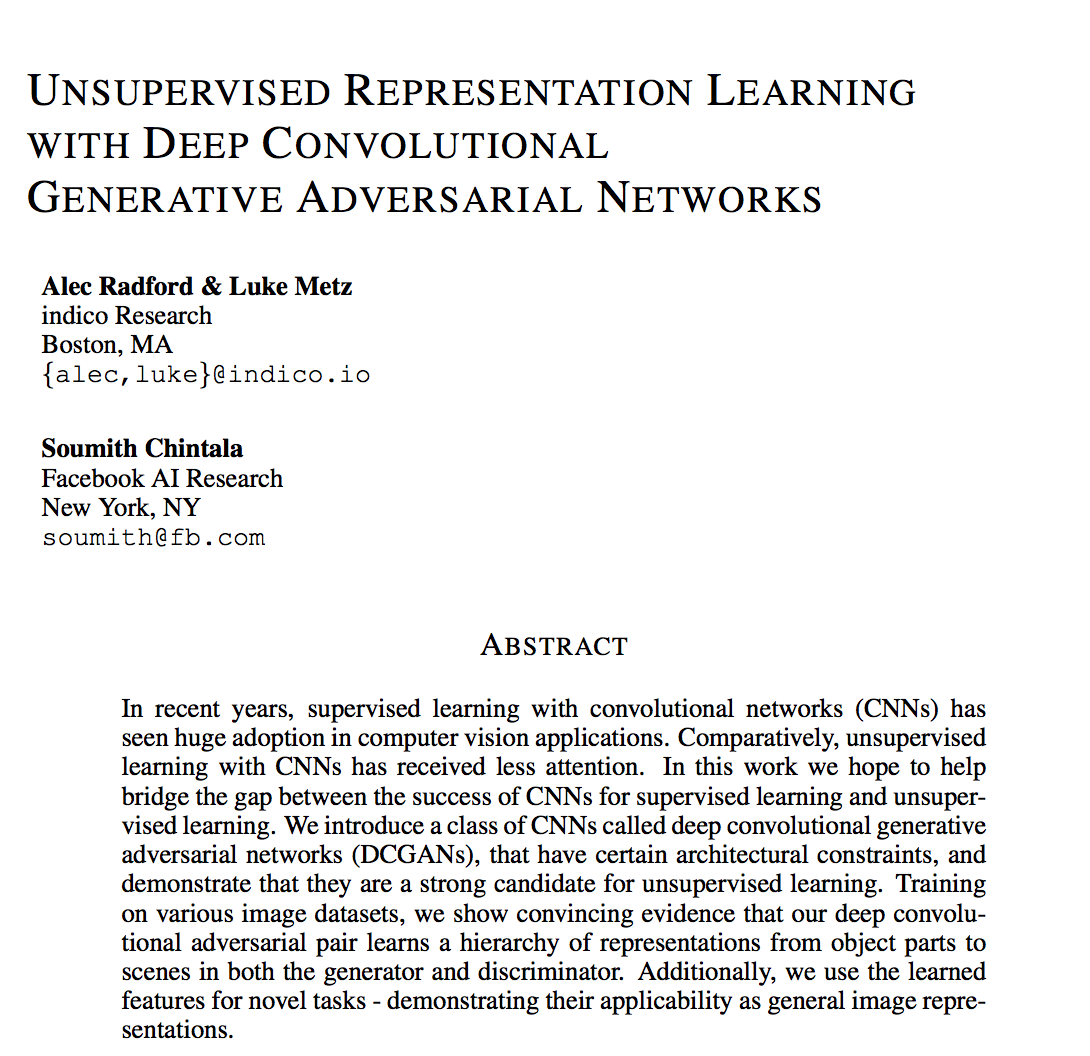
\includegraphics[height=0.9\textheight,keepaspectratio]{images/gan/dcgan-paper.png}
    \end{figure}

    \framebreak

    \begin{figure}
        \centering
        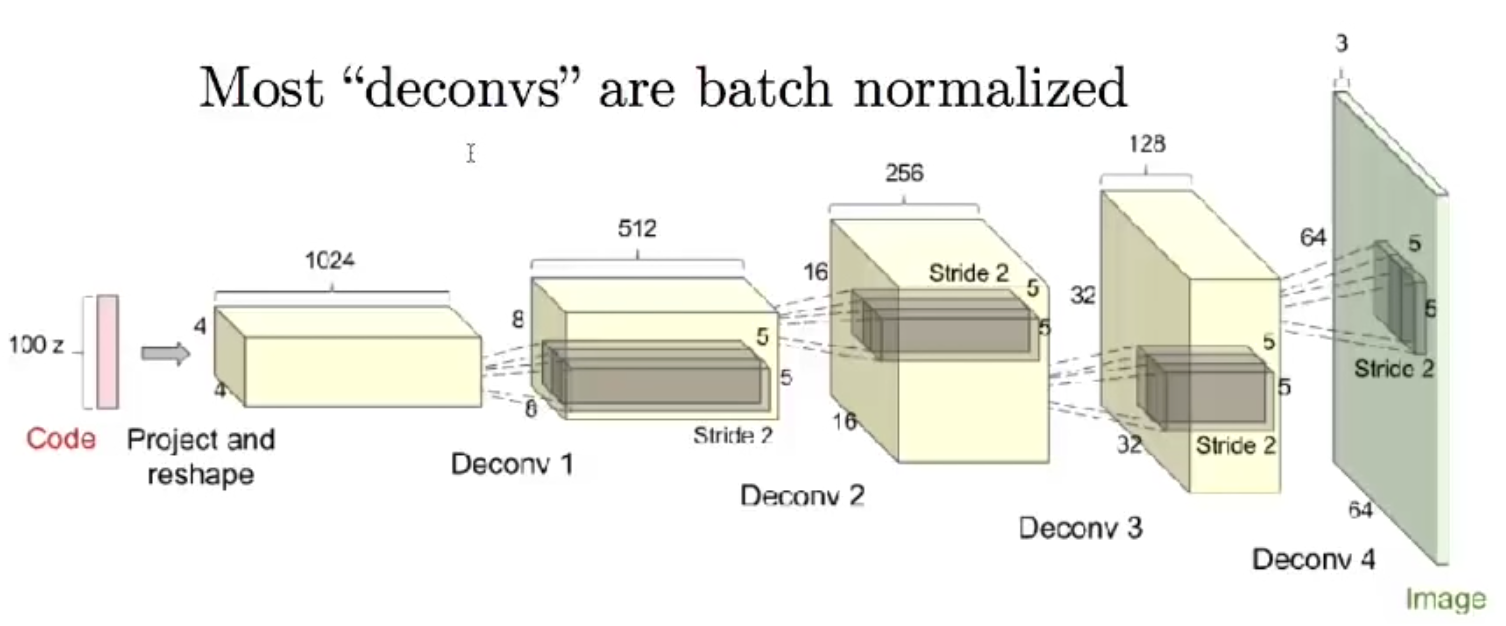
\includegraphics[width=1.05\textwidth,keepaspectratio]{images/gan/dcgan-architecture.png}
        \small [Radford et al 2016]
    \end{figure}

    \framebreak

    \textbf{Architecture Design Principles:}
    \begin{itemize}
        \item Utilizes convolutional and transposed convolutional layers instead of fully connected layers.
        \item Key architectural guidelines:
            \begin{itemize}
                \item Standard supervised CNNs are not directly usable for GANs.
                \item Remove max-pooling and mean-pooling layers.
                \item Generator upsamples using transposed convolutions.
                \item Discriminator downsamples with strided convolutions and average pooling.
                \item Non-linearity: ReLU for generator (except output), LeakyReLU (slope 0.2) for discriminator.
                \item Output non-linearity: \texttt{tanh} for generator, \texttt{sigmoid} for discriminator.
                \item Batch normalization is used to prevent mode collapse, but not applied at the output of G or input of D.
            \end{itemize}
        \item \textbf{Optimization}: Adam optimizer with learning rate $2 \times 10^{-4}$, momentum $0.5$, batch size $128$.
        \item Achieves stable training and generates high-quality images.
    \end{itemize}
\end{frame}
    
\begin{frame}[allowframebreaks]{DCGAN: Results}
    Good samples on datasets with 3M images (Faces, Bedrooms) for the first time
    \begin{figure}
        \centering
        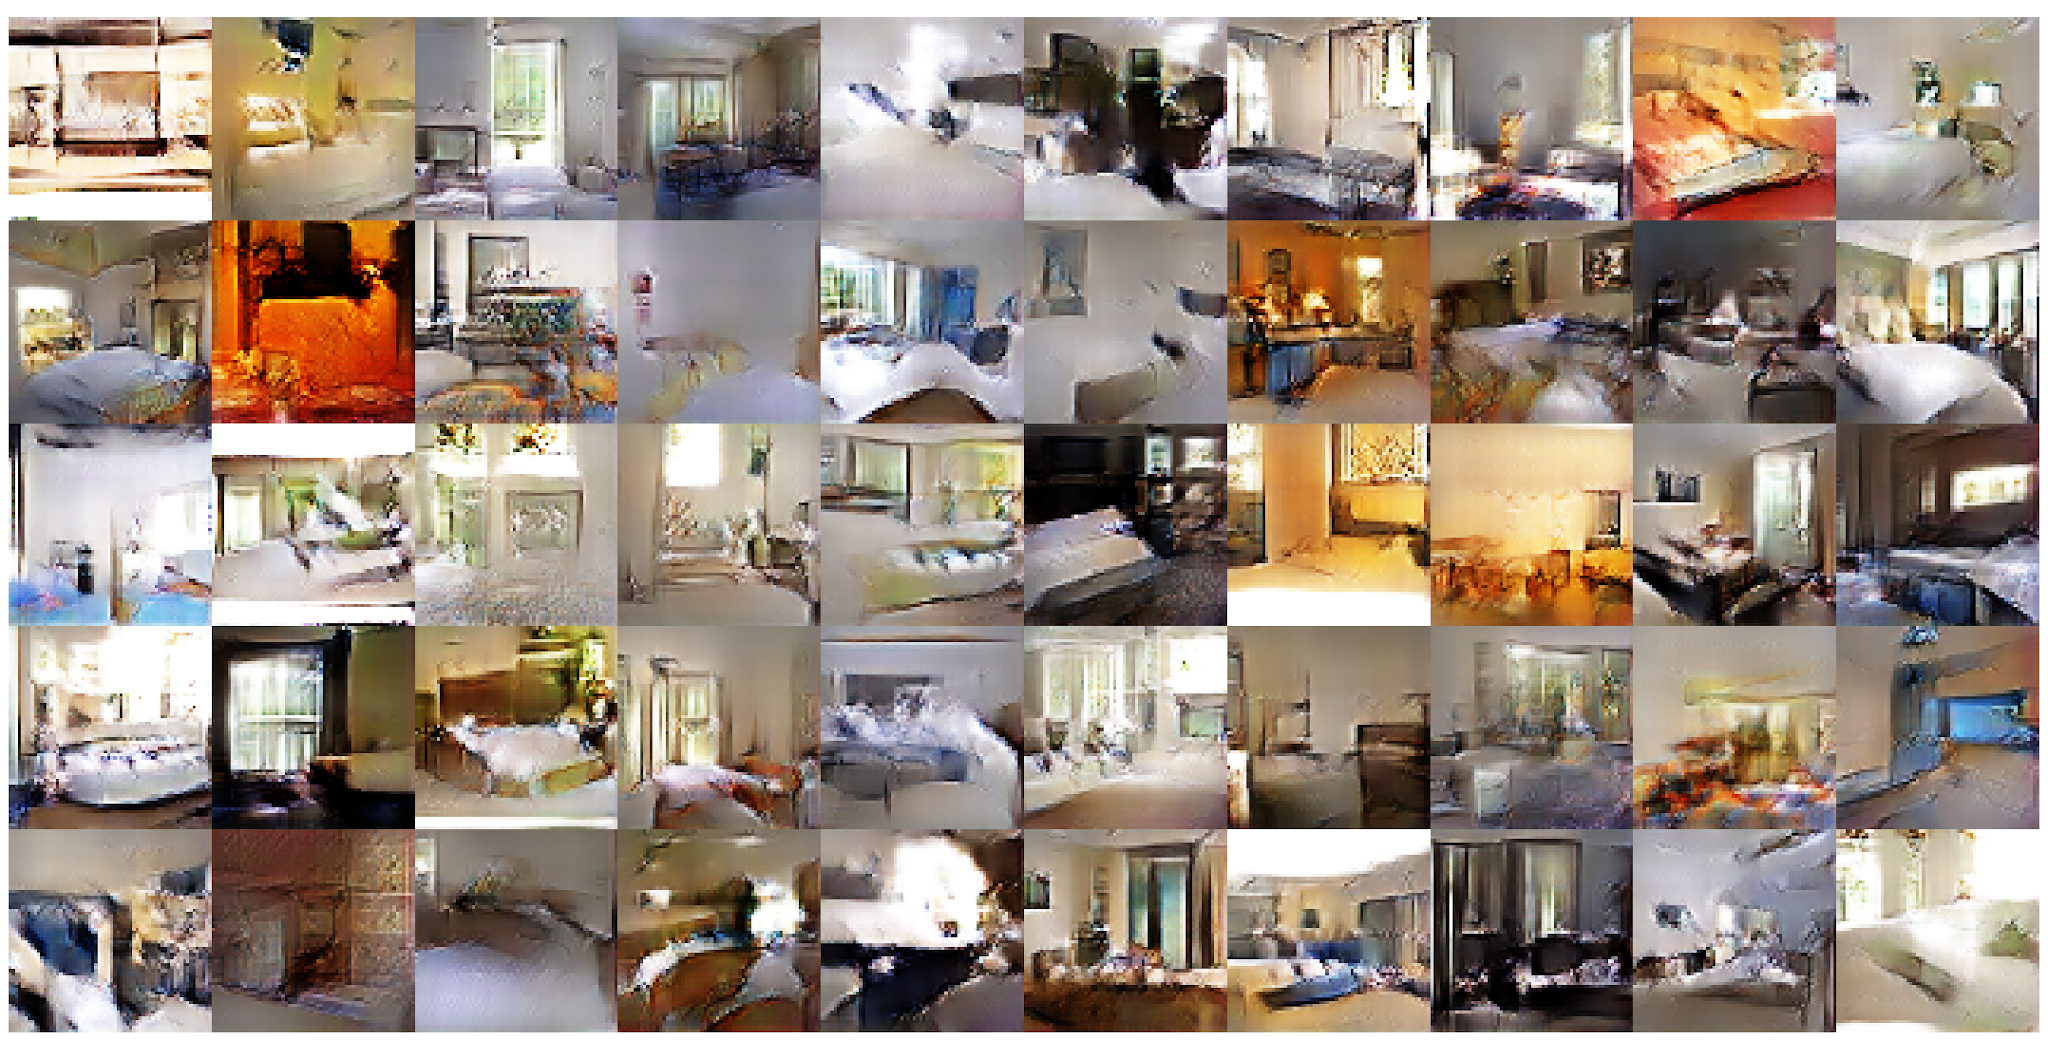
\includegraphics[width=0.9\textwidth,keepaspectratio]{images/gan/dcgan-result-1.png}
    \end{figure}
    \footnotesize{Reference: Radford, Metz, and Chintala, "Unsupervised Representation Learning with Deep Convolutional Generative Adversarial Networks", ICLR 2016}

    \framebreak

    \begin{figure}
        \centering
        \includegraphics[height=0.8\textheight,keepaspectratio]{images/gan/dcgan-result-2.png}
        \caption*{[Radford et al 2016]} 
    \end{figure}

    \framebreak

    Smooth interpolations in high dimensions
    \begin{figure}
        \centering
        \includegraphics[height=0.8\textheight,keepaspectratio]{images/gan/dcgan-result-3.png}
        \caption*{[Radford et al 2016]}
    \end{figure}

    \framebreak

    Imagenet samples (32x32)
    \begin{figure}
        \centering
        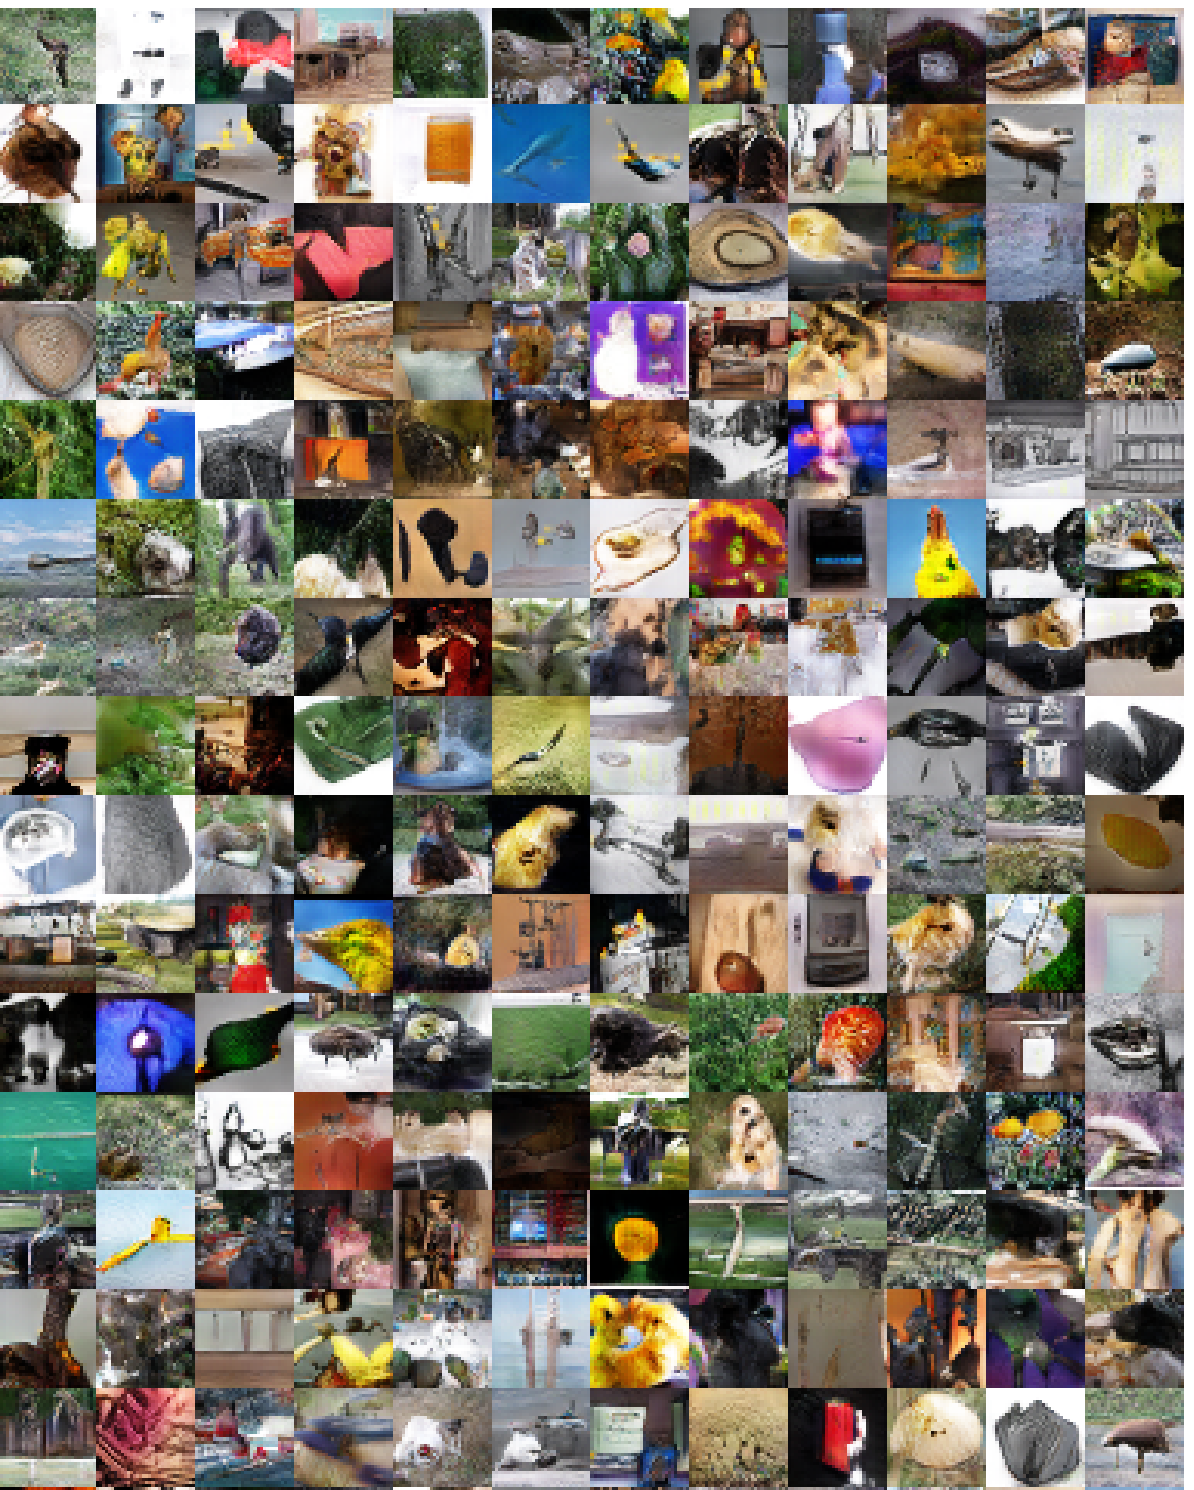
\includegraphics[height=0.8\textheight,keepaspectratio]{images/gan/dcgan-result-4.png}
        \caption*{[Radford et al 2016]}
    \end{figure}

    \framebreak

    Vector Arithmetic
    \begin{figure}
        \centering
        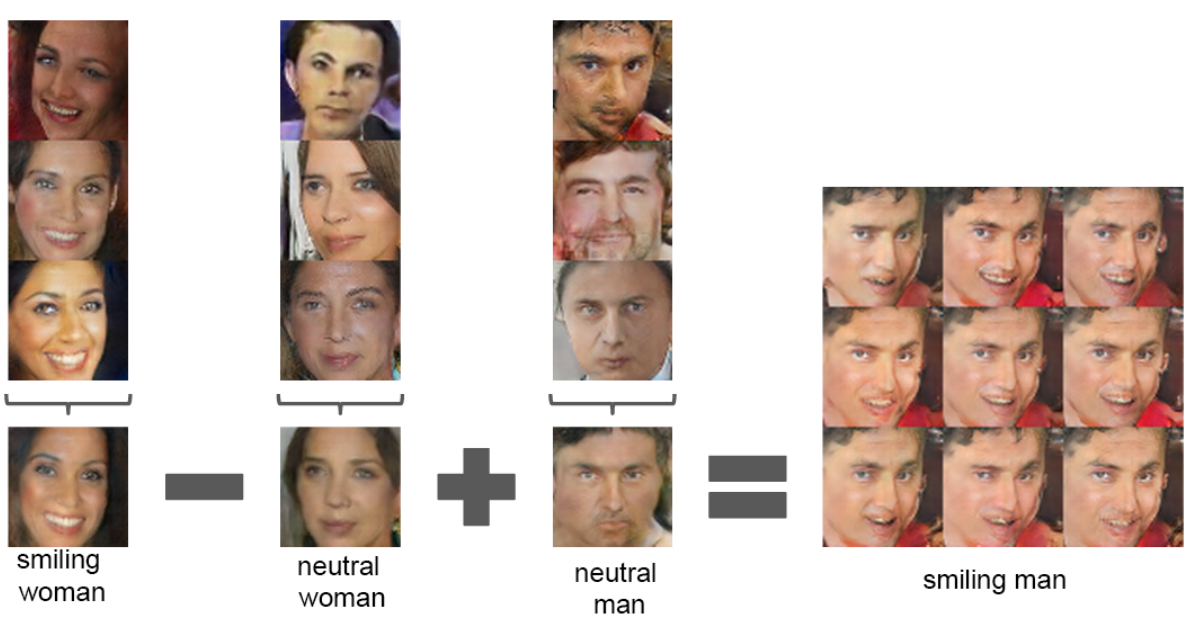
\includegraphics[height=0.75\textheight,keepaspectratio]{images/gan/dcgan-result-5.png}
        \caption*{[Radford et al 2016]}
    \end{figure}

    \framebreak

    \begin{figure}
        \centering
        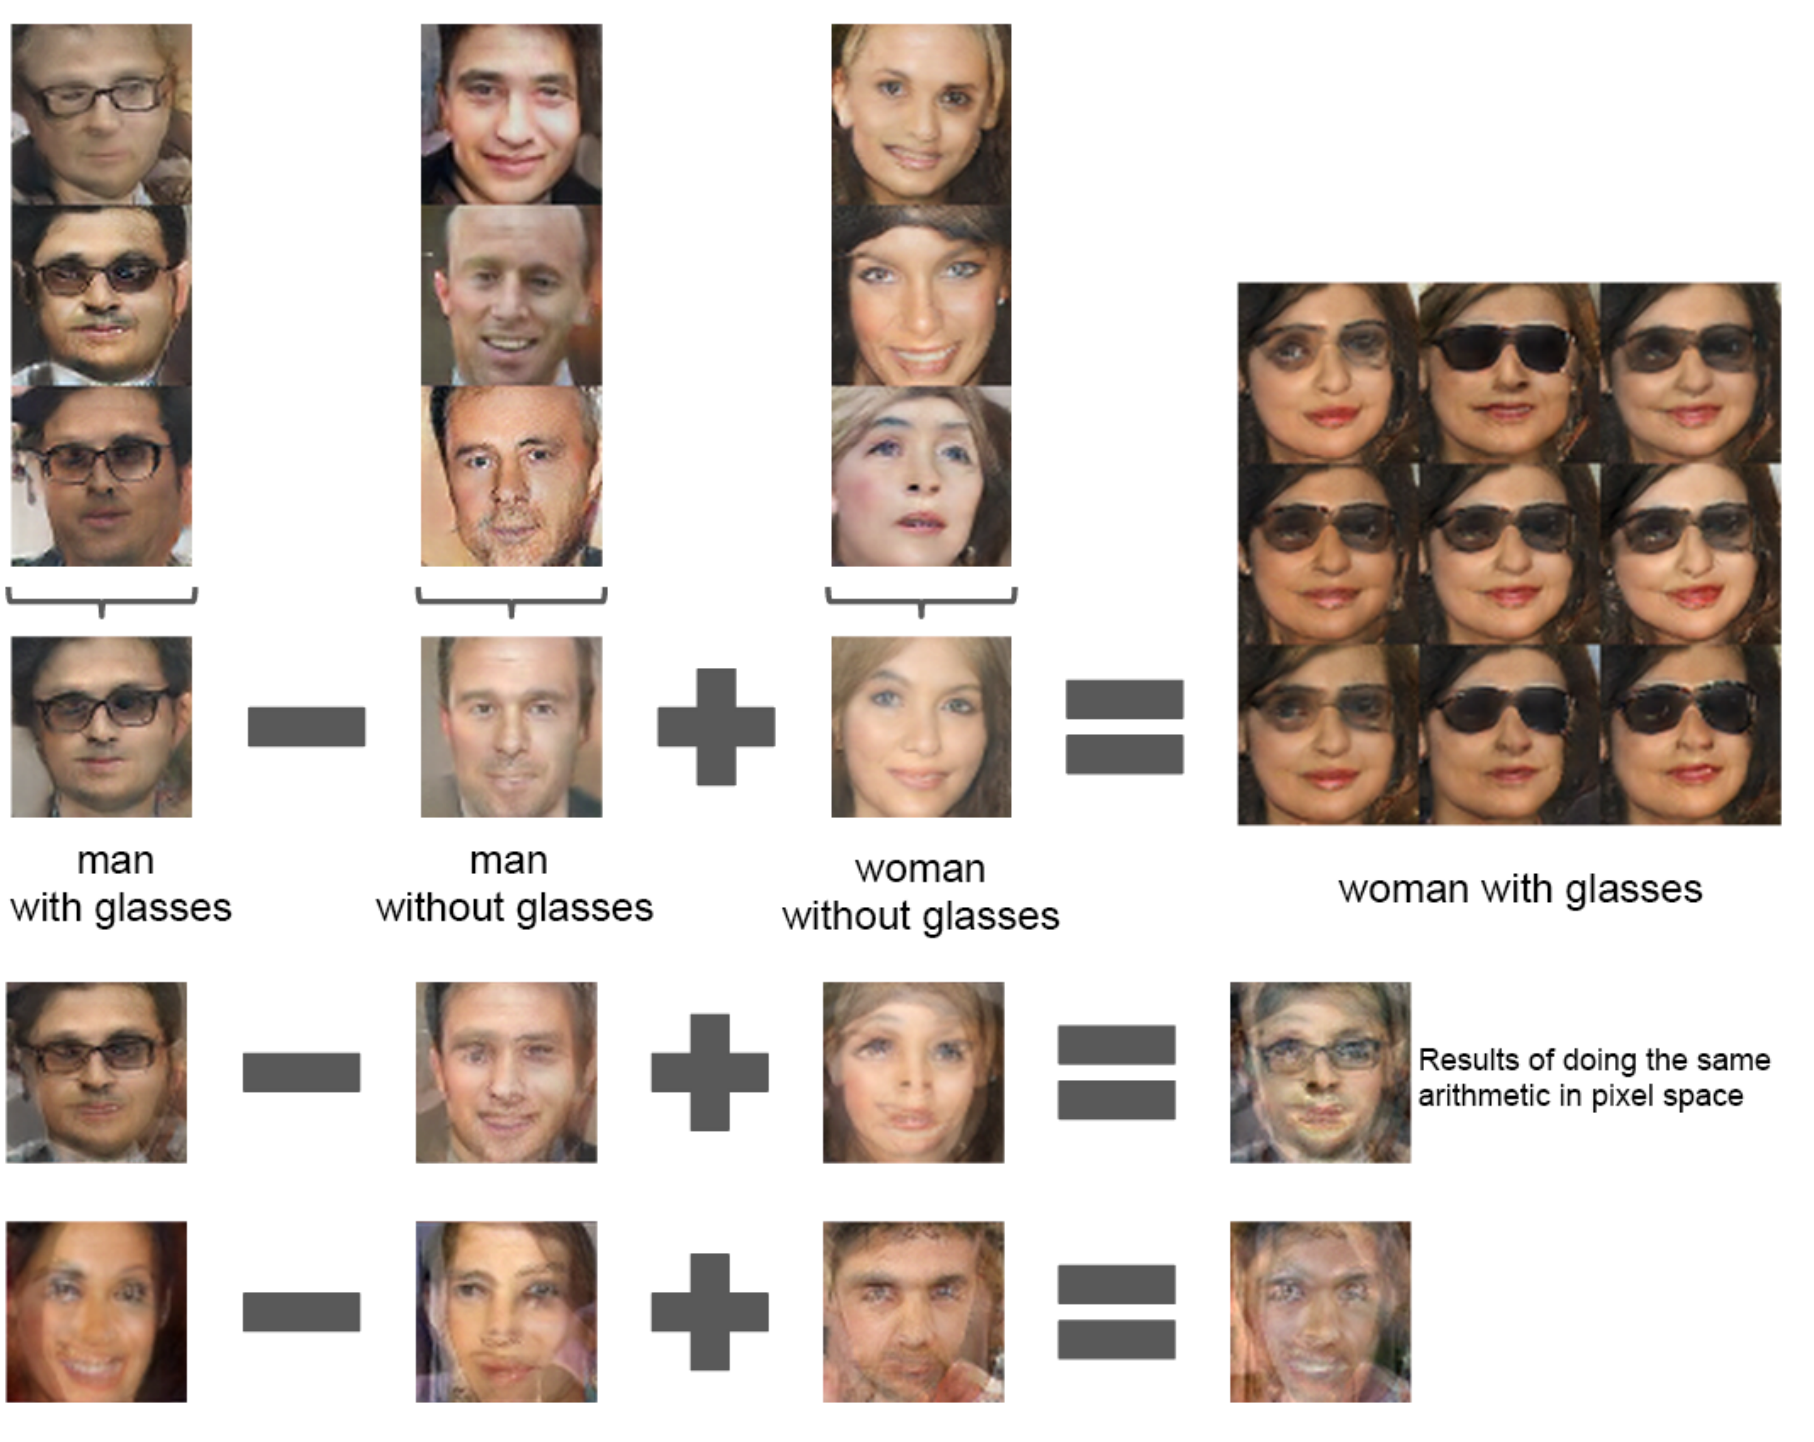
\includegraphics[height=0.8\textheight,keepaspectratio]{images/gan/dcgan-result-6.png}
        \caption*{[Radford et al 2016]}
    \end{figure}

    \framebreak

    \begin{figure}
        \centering
        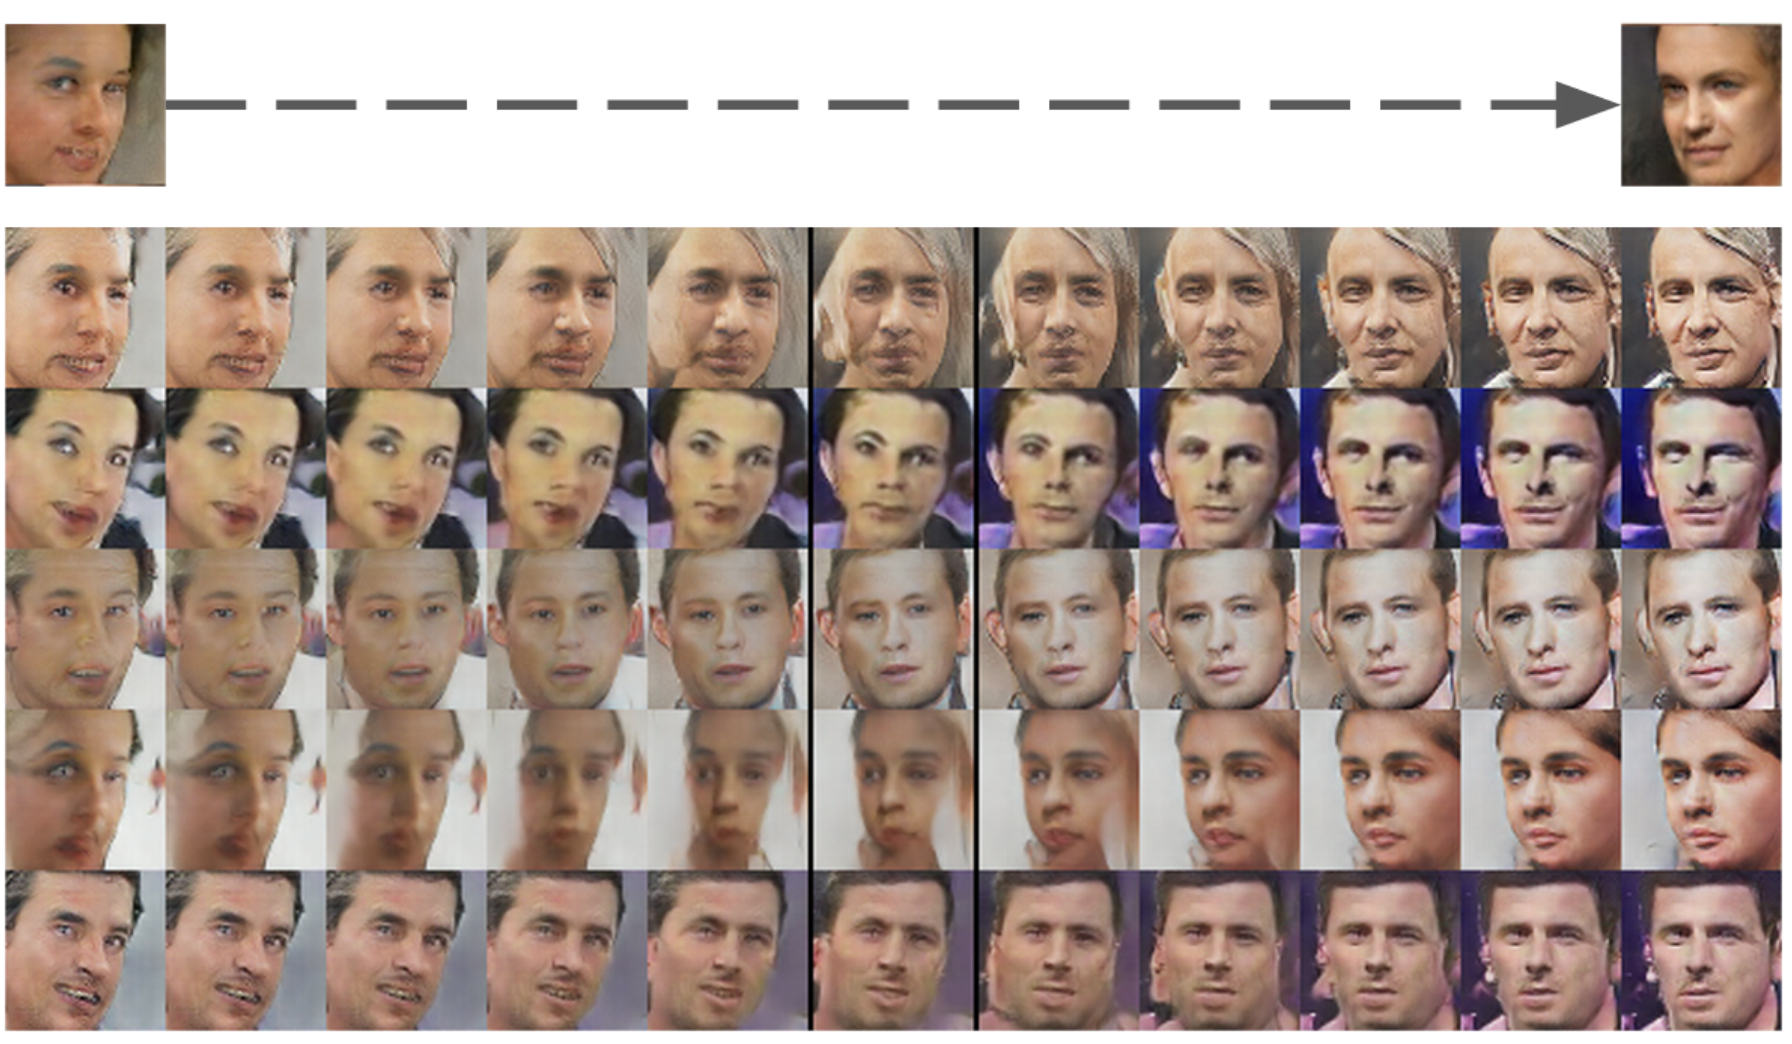
\includegraphics[height=0.8\textheight,keepaspectratio]{images/gan/dcgan-result-7.png}
        \caption*{[Radford et al 2016]}
    \end{figure}

    \framebreak

    Representation Learning 
    \begin{figure}
        \centering
        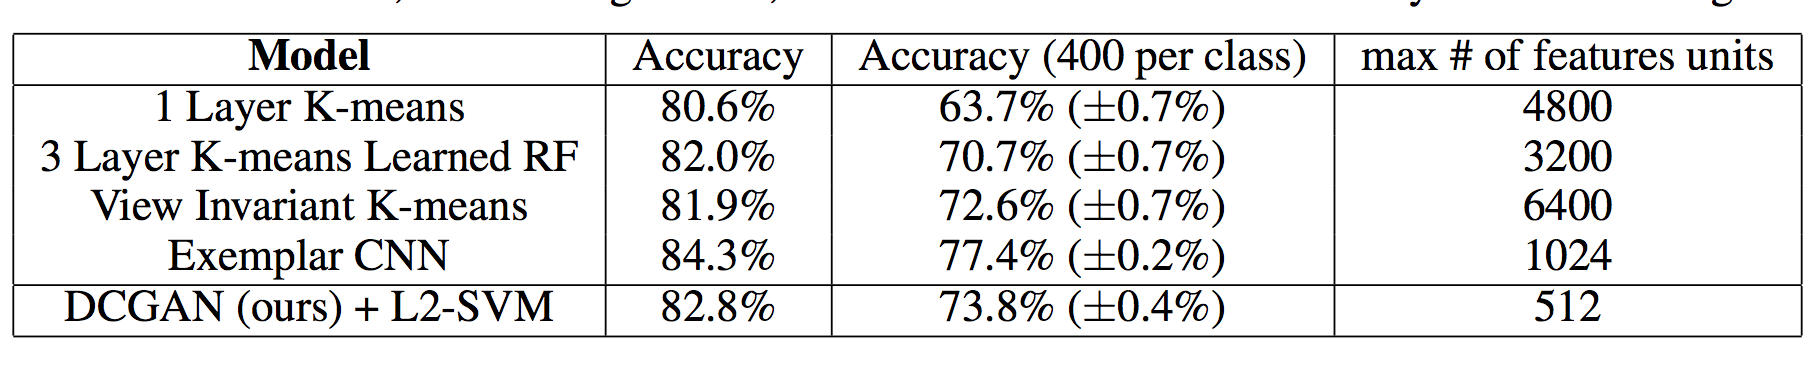
\includegraphics[width=1.05\textwidth,keepaspectratio]{images/gan/dcgan-result-table.png}
        \caption*{[Radford et al 2016]}
    \end{figure}
\end{frame}
\begin{frame}{}
    \LARGE GAN Variant: \\[1.5ex] \textbf{Wasserstein GANs (WGANs)}
\end{frame}

\begin{frame}[allowframebreaks]{Wasserstein GAN}
\begin{itemize}
    \item Wasserstein GAN uses wasserstein distance instead of crossentropy loss.
    \item Wasserstein distance that has a smoother gradient everywhere.
        \begin{figure}
            \centering
            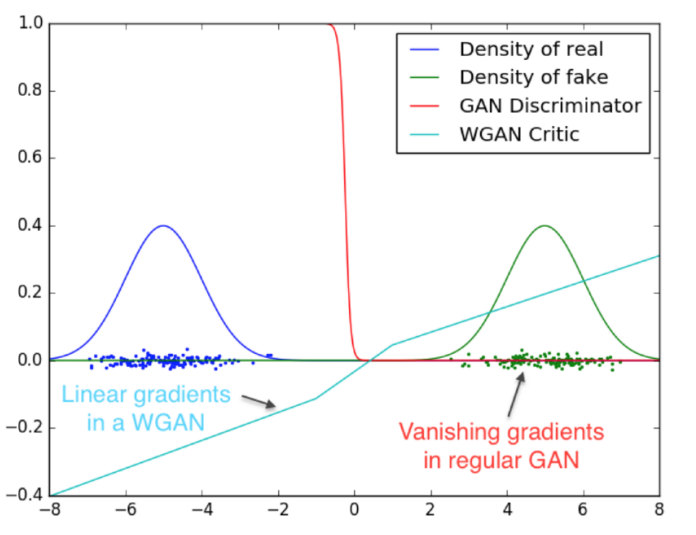
\includegraphics[height=0.6\textheight, width=\textwidth, keepaspectratio]{images/gan/wgan_1.png}
        \end{figure}
\end{itemize}
    
\end{frame}

\begin{frame}{Wasserstein Distance}
\begin{itemize}
    \item Intuitively, it is the shovels of earth moved to make two distributions look alike.
    \begin{figure}
        \centering
        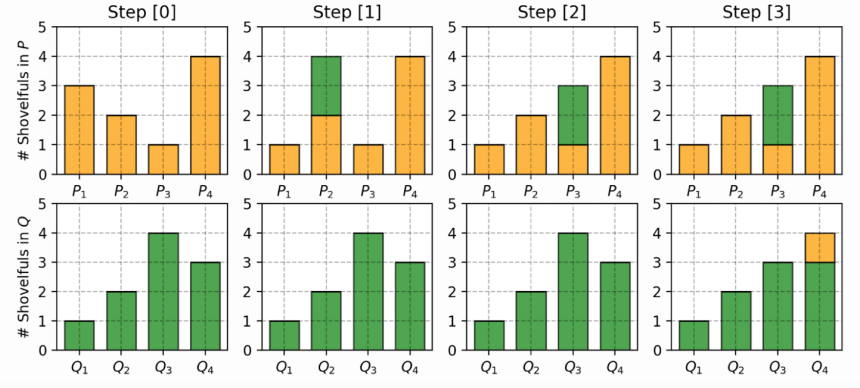
\includegraphics[height=0.6\textheight, width=\textwidth, keepaspectratio]{images/gan/wgan_2.png}
        \caption*{Step by Step plan of moving dirt between piles $P$ and $Q$ to make them match}
    \end{figure}
    
\end{itemize}
    
\end{frame}

\begin{frame}[allowframebreaks]{WGAN}
\begin{figure}
    \centering
    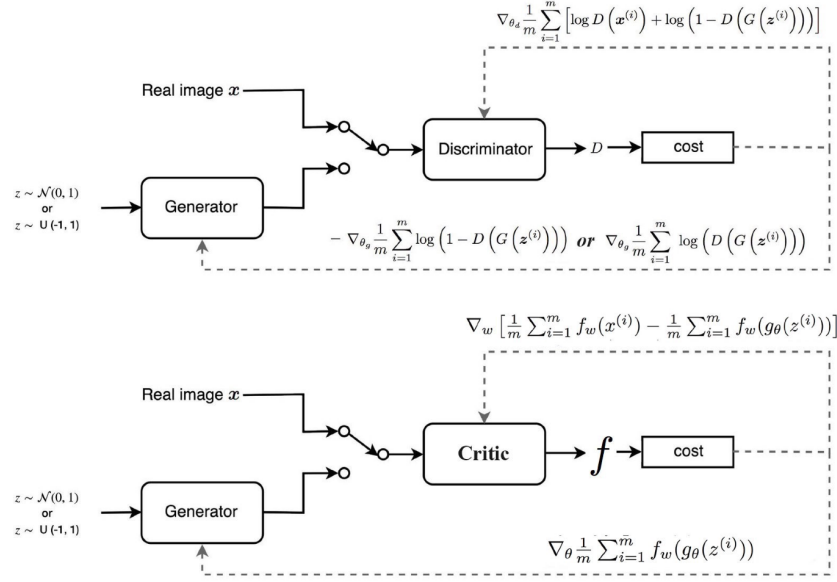
\includegraphics[height=0.9\textheight, width=\textwidth, keepaspectratio]{images/gan/wgan_3.png}
\end{figure}

\framebreak
\begin{figure}
    \centering
    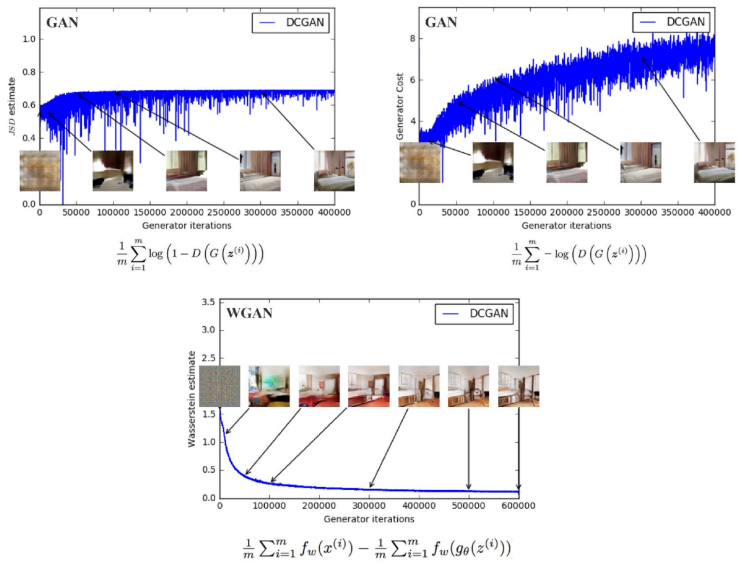
\includegraphics[height=0.9\textheight, width=\textwidth, keepaspectratio]{images/gan/wgan_4.png}
\end{figure}

\framebreak
\begin{figure}
    \centering
    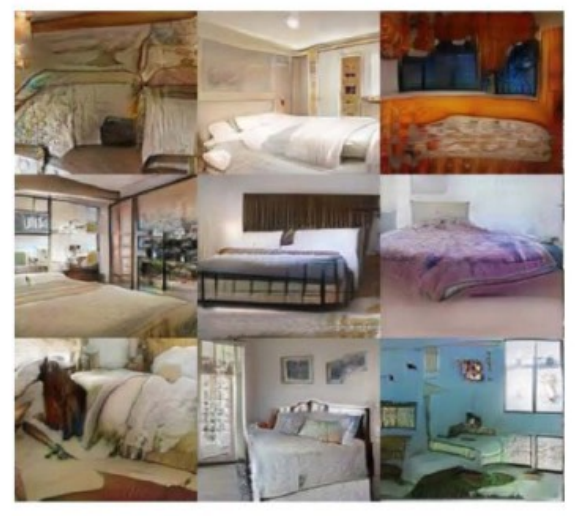
\includegraphics[height=0.8\textheight, width=\textwidth, keepaspectratio]{images/gan/wgan_5.png}
    \caption*{WGAN generation results on bedroom images}
\end{figure}

\end{frame}

\begin{frame}[allowframebreaks]{WGAN-GP: Gradient Penalty for Lipschitzness}
\begin{figure}
    \centering
    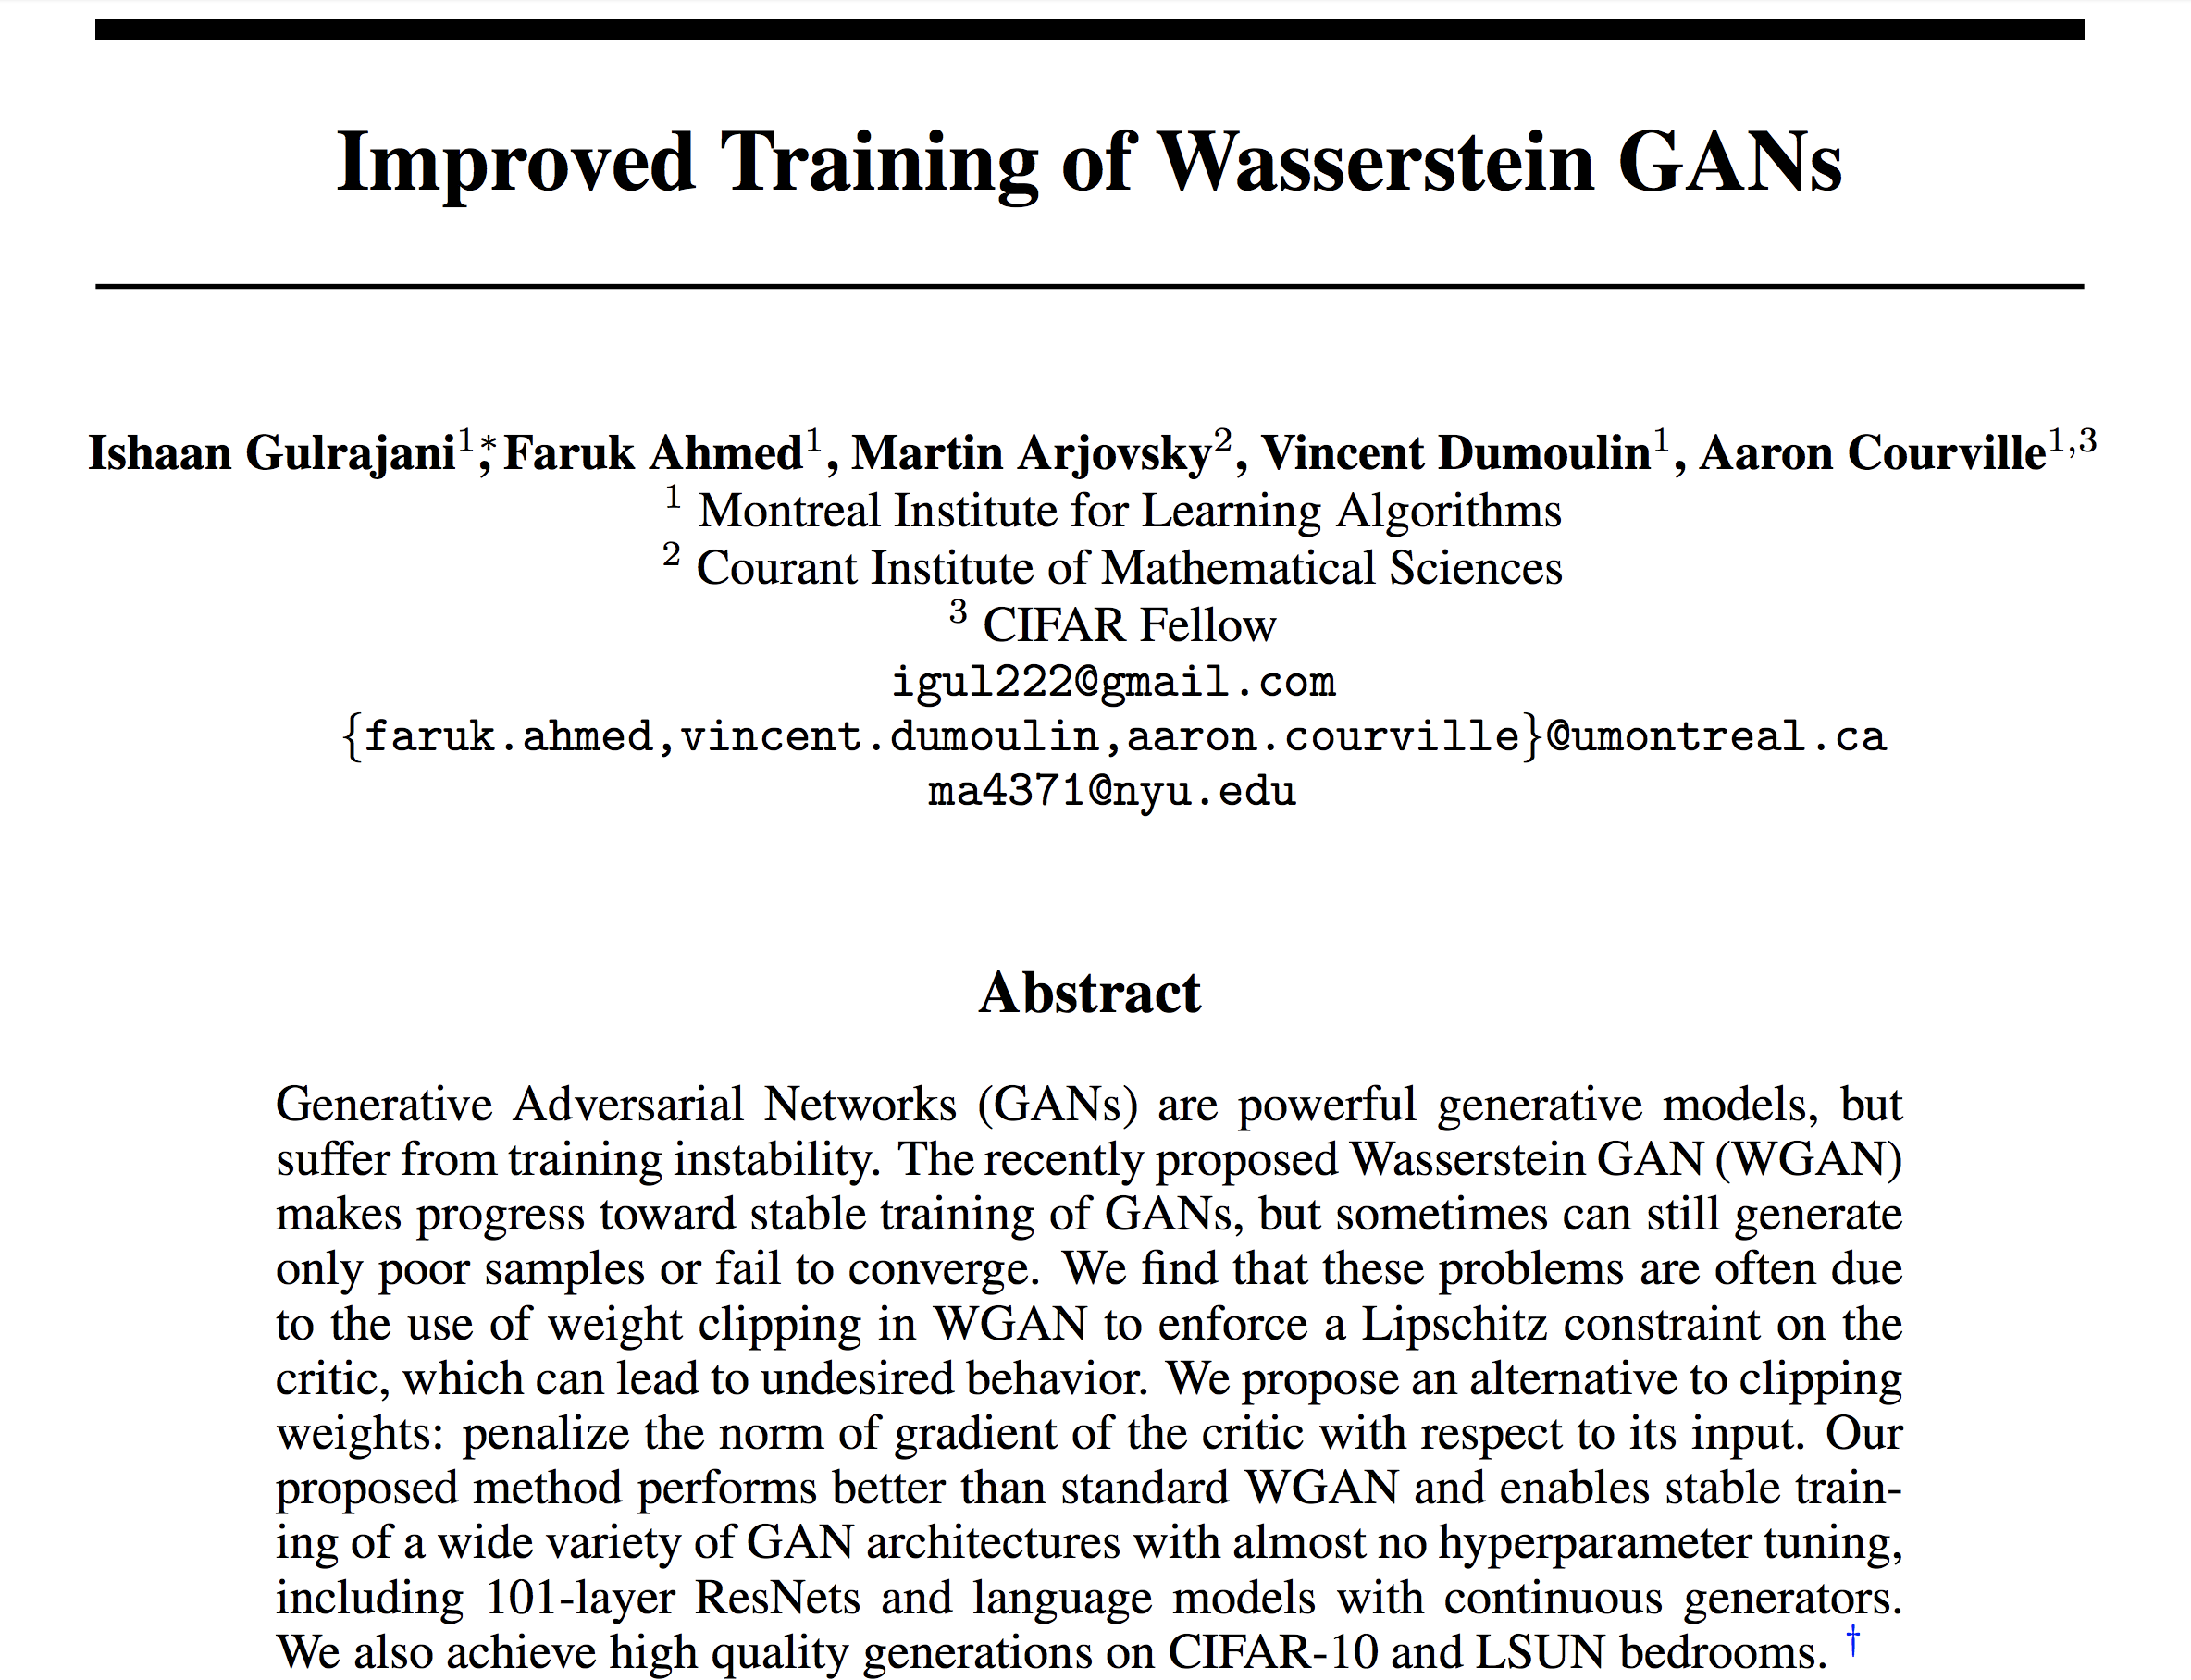
\includegraphics[height=0.8\textheight, width=\textwidth, keepaspectratio]{images/gan/wgan-gp/slide_84_1_img.png}
    \caption*{[Gulrajani et al 2017]}
\end{figure}

\framebreak
\begin{columns}
    \column{0.6\textwidth}
    \begin{figure}
        \centering
        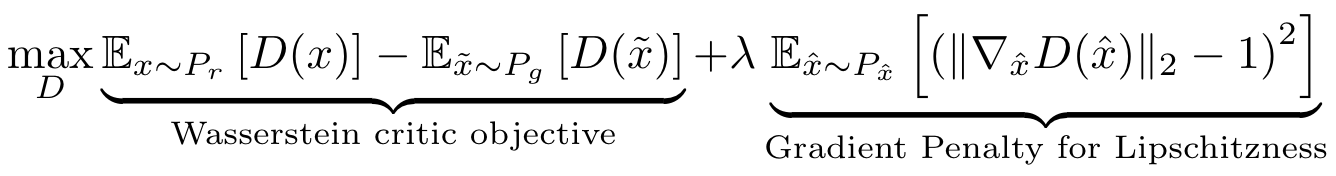
\includegraphics[height=0.8\textheight, width=\textwidth, keepaspectratio]{images/gan/wgan-gp/slide_85_3_img.png}
    \end{figure}
    \begin{figure}
        \centering
        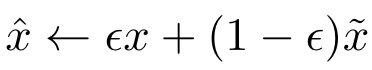
\includegraphics[height=0.1\textheight, width=\textwidth, keepaspectratio]{images/gan/wgan-gp/slide_85_4_img.png}
    \end{figure}
    \column{0.5\textwidth}
    \begin{figure}
        \centering
        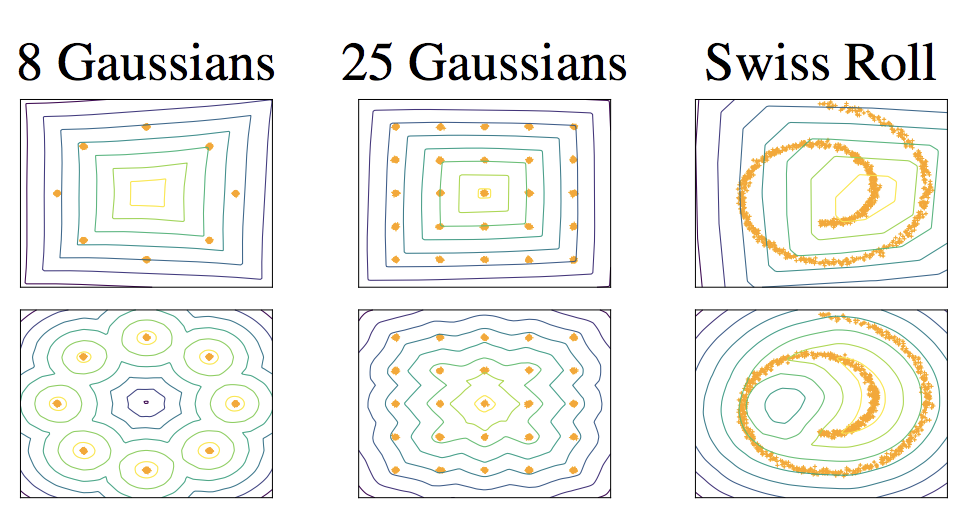
\includegraphics[height=0.8\textheight, width=1.05\textwidth, keepaspectratio]{images/gan/wgan-gp/slide_85_2_img.png}
    \end{figure}
    \begin{figure}
        \centering
        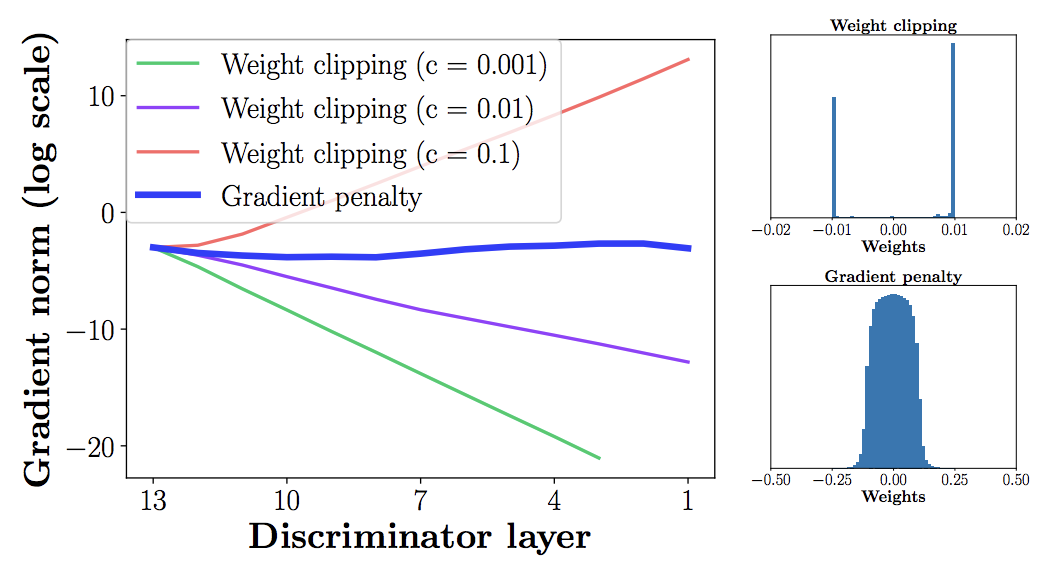
\includegraphics[height=0.8\textheight, width=1.05\textwidth, keepaspectratio]{images/gan/wgan-gp/slide_85_1_img.png}
    \end{figure}
\end{columns}
\end{frame}

\begin{frame}[allowframebreaks]{WGAN-GP: Pseudocode}
    \begin{figure}
        \centering
        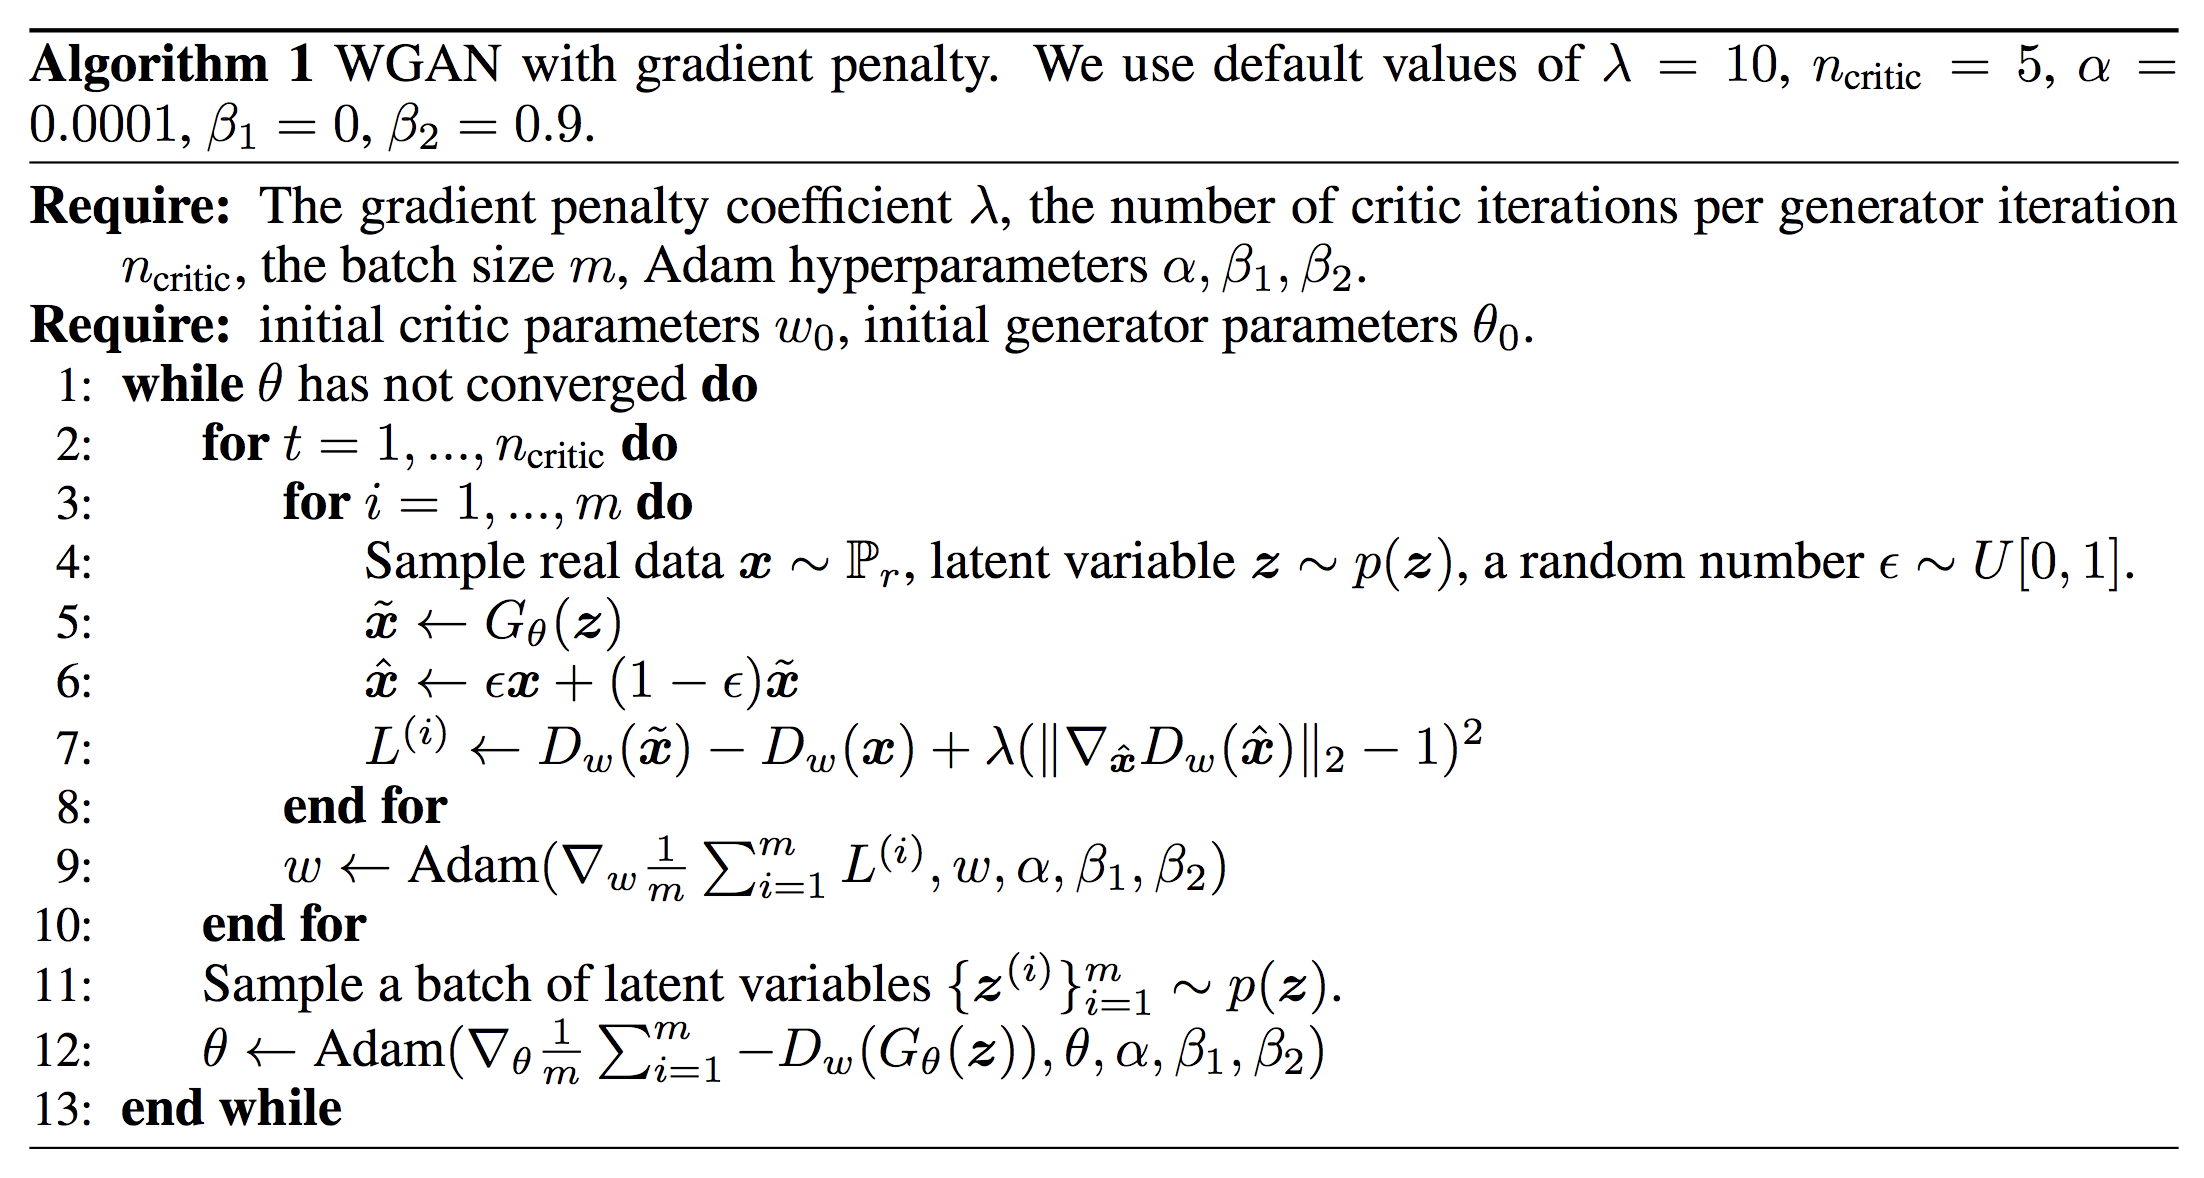
\includegraphics[height=0.8\textheight, width=1.05\textwidth, keepaspectratio]{images/gan/wgan-gp/slide_86_1_img.png}
        \caption*{[Gulrajani et al 2017]}
    \end{figure}
\end{frame}

\begin{frame}[allowframebreaks]{WGAN-GP: BatchNorm}
    \begin{figure}
        \centering
        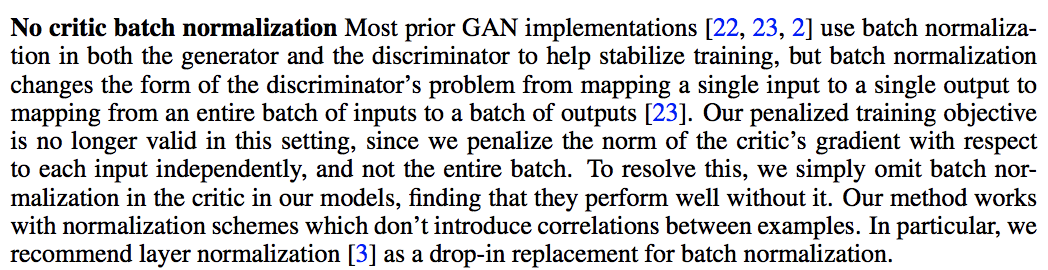
\includegraphics[height=0.8\textheight, width=1.05\textwidth, keepaspectratio]{images/gan/wgan-gp/slide_87_1_img.png}
        \caption*{[Gulrajani et al 2017]}
    \end{figure}
\end{frame}

\begin{frame}[allowframebreaks]{WGAN-GP: Robustness to architectures}
    \begin{figure}
        \centering
        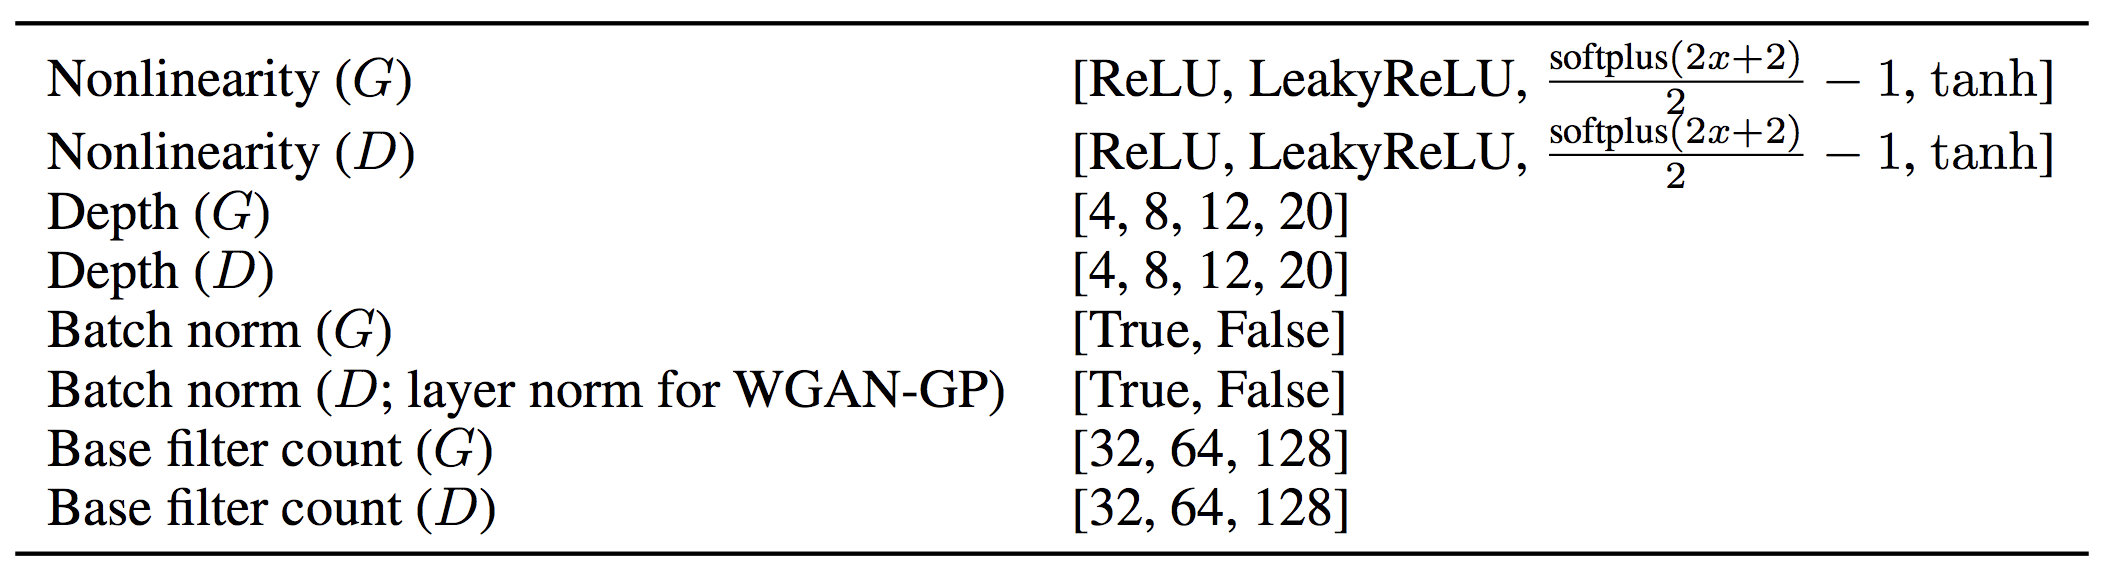
\includegraphics[height=0.8\textheight, width=1.05\textwidth, keepaspectratio]{images/gan/wgan-gp/slide_88_1_img.png}
    \end{figure}
    \begin{figure}
        \centering
        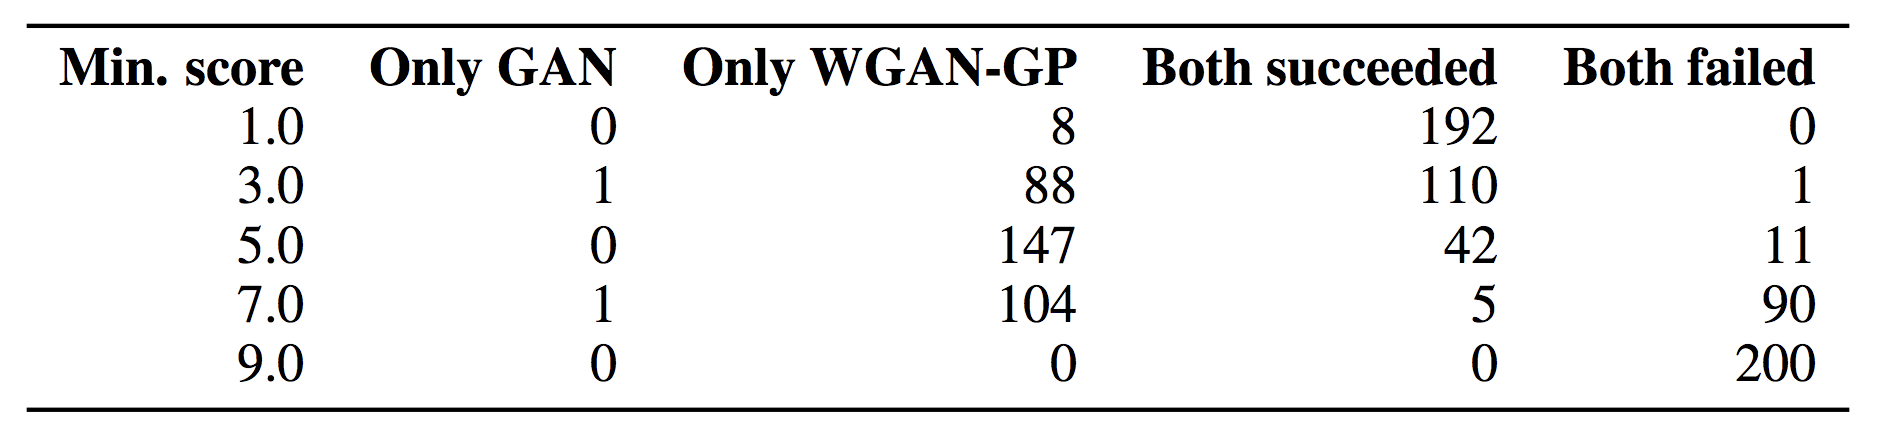
\includegraphics[height=0.8\textheight, width=1.05\textwidth, keepaspectratio]{images/gan/wgan-gp/slide_88_2_img.png}
        \caption*{[Gulrajani et al 2017]}
    \end{figure}

    \framebreak

    \begin{figure}
        \centering
        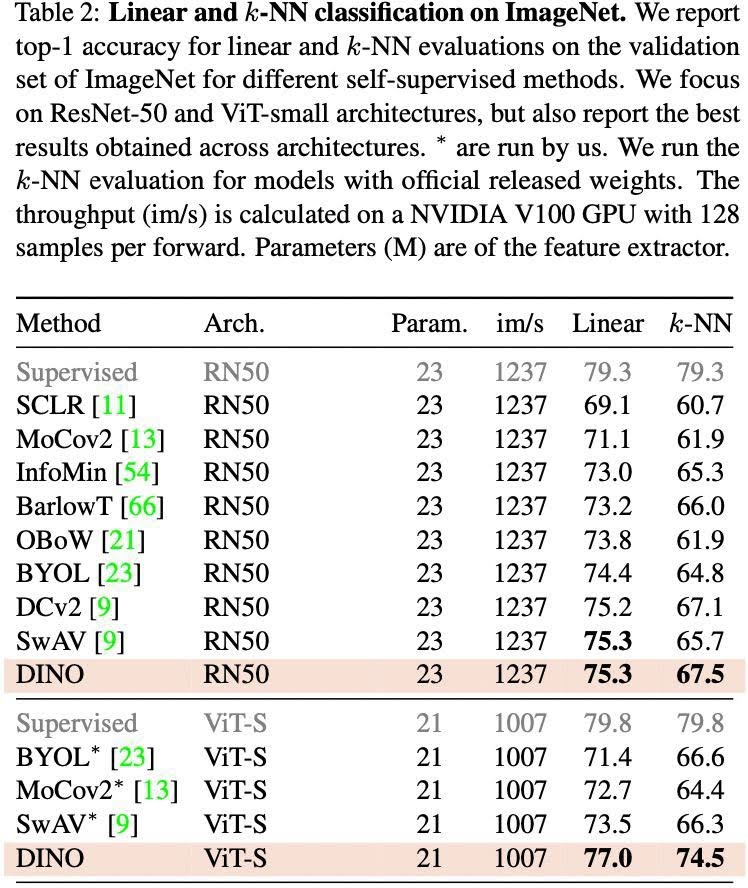
\includegraphics[height=0.85\textheight, width=1.05\textwidth, keepaspectratio]{images/gan/wgan-gp/slide_89_1_img.png}
        \caption*{[Gulrajani et al 2017]}
    \end{figure}
\end{frame}


\begin{frame}[allowframebreaks]{WGAN-GP: High quality samples}
    \begin{figure}
        \centering
        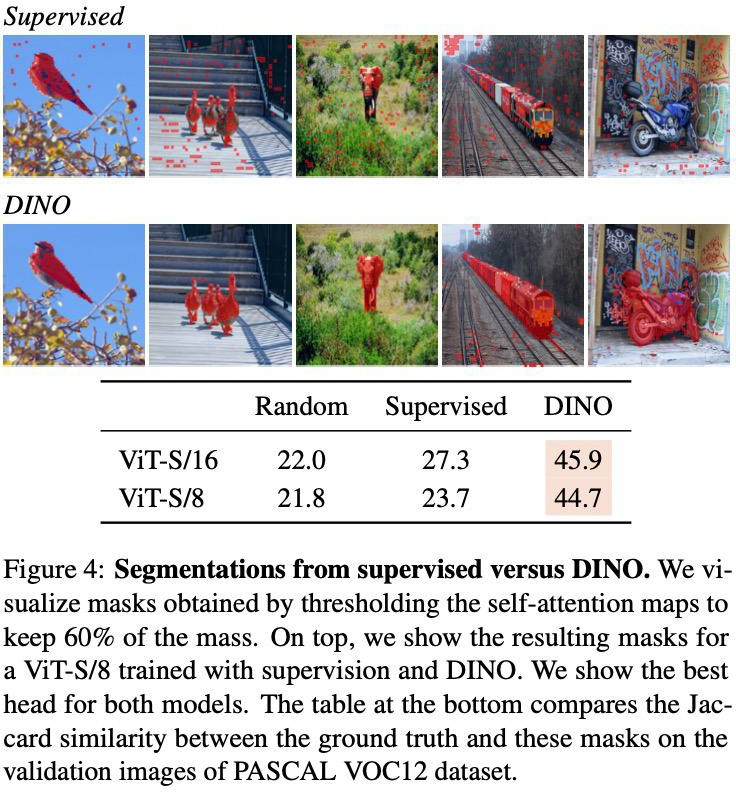
\includegraphics[height=0.8\textheight, width=1.05\textwidth, keepaspectratio]{images/gan/wgan-gp/slide_90_1_img.png}
        \caption*{[Gulrajani et al 2017]}
    \end{figure}

    \framebreak

    \begin{figure}
        \centering
        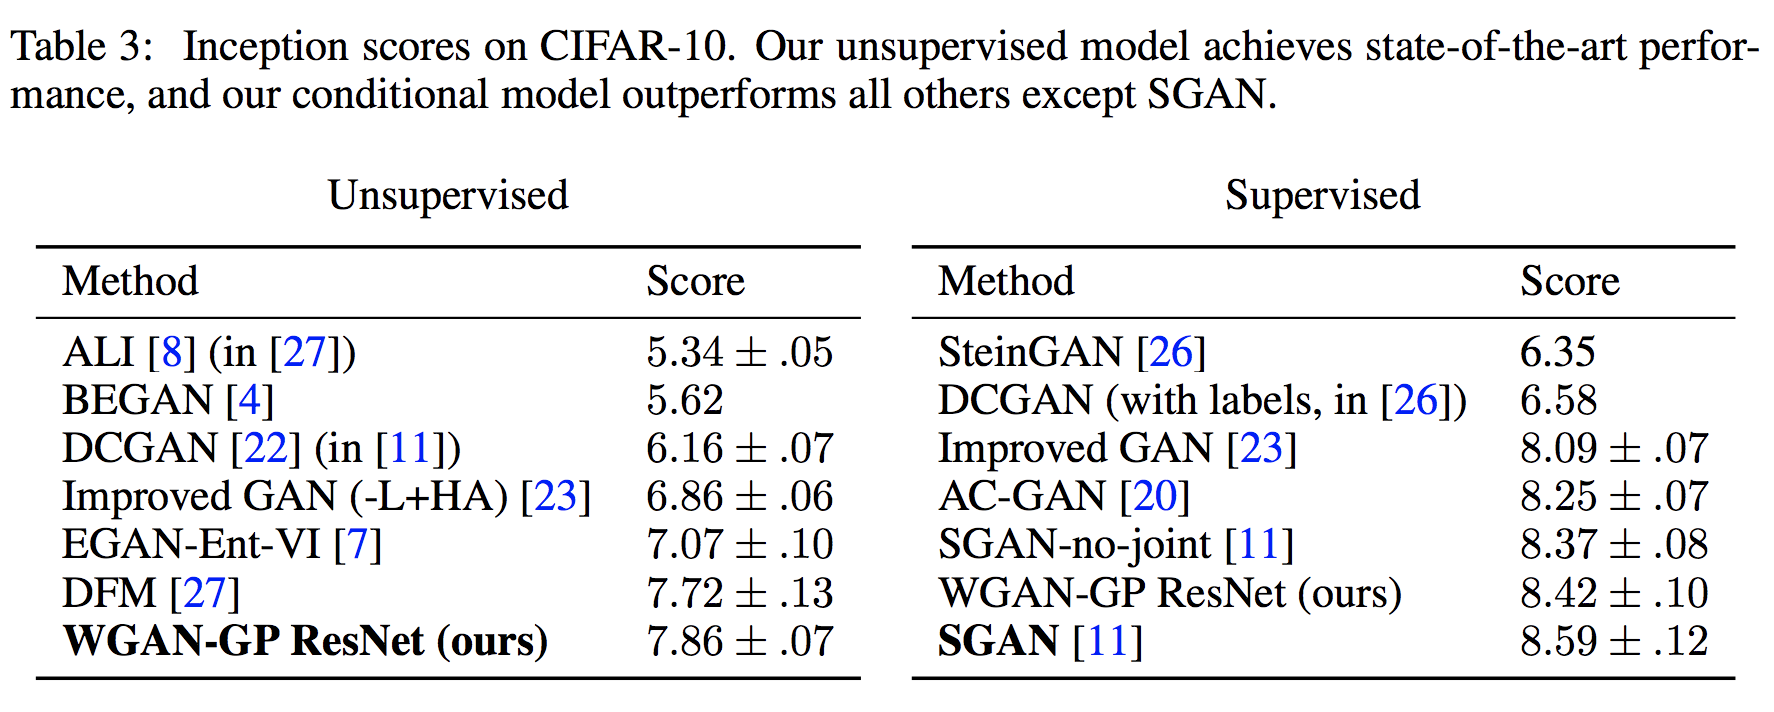
\includegraphics[height=0.8\textheight, width=1.05\textwidth, keepaspectratio]{images/gan/wgan-gp/slide_91_1_img.png}
        \caption*{[Gulrajani et al 2017]}
    \end{figure}
\end{frame}
\begin{frame}[allowframebreaks]{Conditional GAN}
\begin{itemize}
    \item In addition to random noise, a condition is added to the generator input. 
    \item The discriminator also receives this condition.
\end{itemize}
\begin{figure}
    \centering
    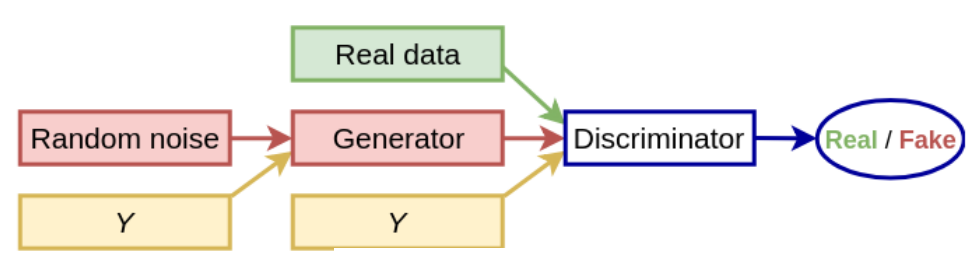
\includegraphics[height=0.8\textheight, width=\textwidth, keepaspectratio]{images/gan/cond_gan_1.png}
\end{figure}

\framebreak
\begin{itemize}
    \item Discriminator Loss:
    \begin{align*}
    \mathcal{L}^{(D)} \left( \theta^{(G)}, \theta^{(D)} \right) =\ & 
    - \mathbb{E}_{x \sim p_{data}} \left[ \log D(x|y) \right] \\
    & - \mathbb{E}_{z \sim p_z(z),\ y \sim p_{data}(y)} \left[ \log(1 - D(G(z|y))) \right]
    \end{align*}
    \item Generator Loss:
    $$
    \mathcal{L}^{(G)} \left( \theta^{(G)}, \theta^{(D)} \right) = - \mathbb{E}_z \left[ \log D(G(z|y)) \right]
    $$
\end{itemize}

\framebreak
\begin{figure}
    \centering
    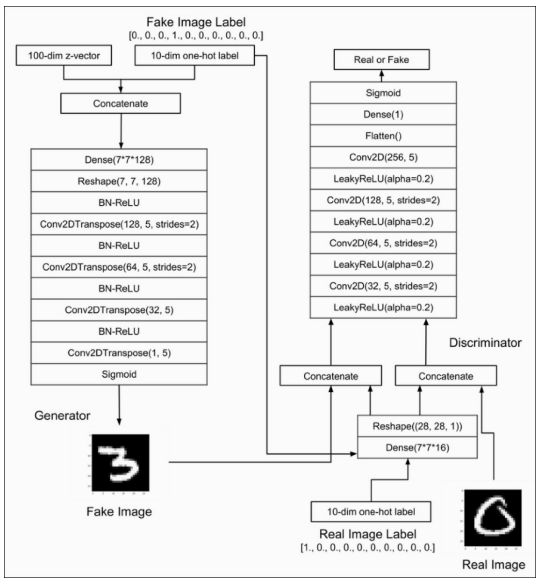
\includegraphics[height=0.8\textheight, width=\textwidth, keepaspectratio]{images/gan/cond_gan_2.png}
    \caption{A conditional GAN architecture for the MNIST digits dataset.}
\end{figure}

\end{frame}

\begin{frame}[allowframebreaks]{Condional GAN - Image to Image}

\begin{figure}
    \centering
    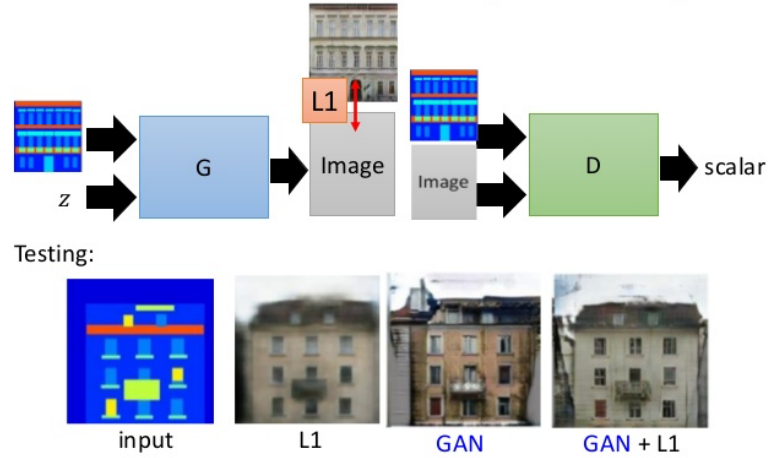
\includegraphics[height=0.75\textheight, width=\textwidth, keepaspectratio]{images/gan/cond_gan_3.png}
    \caption{Using L1 loss in addition in GAN loss can help in image to image translation}
\end{figure}

\framebreak

\begin{figure}
    \centering
    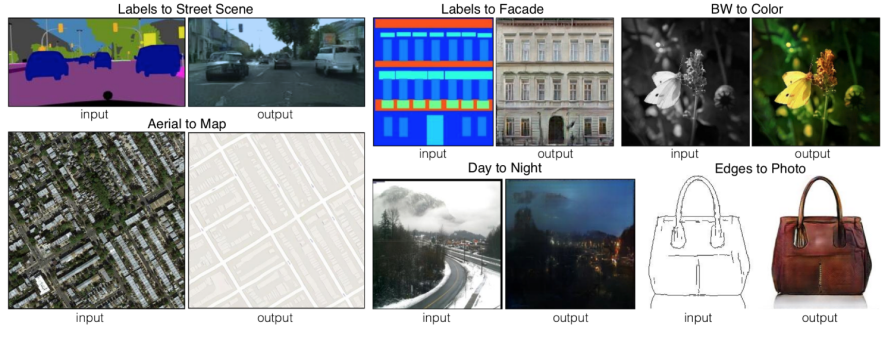
\includegraphics[height=0.8\textheight, width=\textwidth, keepaspectratio]{images/gan/cond_gan_4.png}
    \caption{Image to Image translation with condional GANs}
\end{figure}
    
\end{frame}
\subsection{Pix2Pix GANs}
\begin{frame}{}
    \LARGE GAN Variant: \\[1.5ex] \textbf{Pix2Pix GANs}
\end{frame}

\begin{frame}[allowframebreaks]{Pix2Pix GANs}
    \textbf{Motivation:}

    \begin{itemize}
        \item Many computer vision tasks require translating one type of image to another:
        \begin{itemize}
            \item Sketch $\rightarrow$ Photo
            \item Day $\rightarrow$ Night
            \item Black \& white $\rightarrow$ Color
            \item Aerial photo $\rightarrow$ Map
        \end{itemize}
        \item Traditional methods rely on paired datasets (input-output examples), manual labeling, or hand-crafted heuristics.
        \item Generative Adversarial Networks (GANs) have shown great success in generating realistic images.
        \item Conditional GANs (cGANs) extend GANs to perform image-to-image translation by conditioning on input images.
    \end{itemize}
\framebreak
    \textbf{What is Pix2Pix?}

    \begin{itemize}
        \item Pix2Pix is a Conditional GAN (cGAN) framework for supervised image-to-image translation.
        \item Introduced in the paper: \textit{Image-to-Image Translation with Conditional Adversarial Networks} by Isola et al., 2017.
    \end{itemize}
\framebreak
    \textbf{Architecture:}
    \begin{itemize}
        \item \textbf{Generator (G):} U-Net (encoder-decoder with skip connections) that transforms the input image (e.g., sketch) into the target image (e.g., photo).
        \item \textbf{Discriminator (D):} PatchGAN classifier that determines whether a patch of the image is real or fake, enforcing local realism.
    \end{itemize}

    \begin{figure}
        \centering
        \fetchconvertimage{https://www.researchgate.net/publication/383558465/figure/fig3/AS:11431281274620774@1725036289021/Schema-of-Pix2Pix-GAN-architecture.jpg}{images/gan/pix2pix-architecture.png}{width=1\textwidth,height=0.55\textheight,keepaspectratio}
        % \caption*{Pix2Pix GAN architecture. The generator transforms an input image to a target image, while the discriminator evaluates the realism of the generated output.}
    \end{figure}

    \textbf{How It Works:}
    \begin{itemize}
        \item The generator learns to map an input image to a target image.
        \item The discriminator distinguishes between:
        \begin{itemize}
            \item Real pairs: (input, real output)
            \item Fake pairs: (input, generated output)
        \end{itemize}
        \item \textbf{Loss Function:}
        \begin{itemize}
            \item \textbf{Adversarial Loss:} Encourages the output to look realistic.
            \item \textbf{L1 Loss:} Encourages the output to be close to the target image (pixel-wise similarity).
        \end{itemize}
        \item \textbf{Total Loss:} Adversarial Loss $+$ $\lambda$ $\times$ L1 Loss \\
        ($\lambda$ is a weight to balance realism and similarity)
    \end{itemize}
\framebreak
    \begin{figure}
        \centering
        \fetchconvertimage{https://www.researchgate.net/publication/370213457/figure/fig3/AS:11431281153057998@1682322888544/a-Schematic-of-the-pix2pix-GAN-architecture-for-reconstructing-image-from-noisy-power.png}{images/gan/pix2pix-result-0.png}{width=1\textwidth,height=0.9\textheight,keepaspectratio}
    \end{figure}
\end{frame}

\begin{frame}[allowframebreaks]{Pix2Pix GANs: Results}
    \begin{figure}
        \centering
        \fetchconvertimage{https://phillipi.github.io/pix2pix/images/edges2cats.jpg}{images/gan/pix2pix-result-1.png}{width=1\textwidth,height=0.9\textheight,keepaspectratio,trim={0 {.5\textheight} 0 0},clip}
    \end{figure}
\framebreak
    \begin{figure}
        \centering
        \fetchconvertimage{https://www.tensorflow.org/images/gan/pix2pix_1.png}{images/gan/pix2pix-result-2.png}{width=1\textwidth,height=0.9\textheight,keepaspectratio}
    \end{figure}
\framebreak
    \begin{figure}
        \centering
        \fetchconvertimage{https://machinelearningmastery.com/wp-content/uploads/2019/05/Pix2Pix-GAN-Translation-of-Semantic-Images-to-Photographs-of-a-Cityscape.png}{images/gan/pix2pix-result-3.png}{width=1\textwidth,height=0.9\textheight,keepaspectratio}
    \end{figure}
\end{frame}
\begin{frame}[allowframebreaks]{Cycle GANs}

\begin{itemize}
    \item Unpaired Image-to-Image Translation using Cycle-Consistent Adversarial Networks, Efros, ICC7 2017
    
\end{itemize}
\begin{figure}
    \centering
    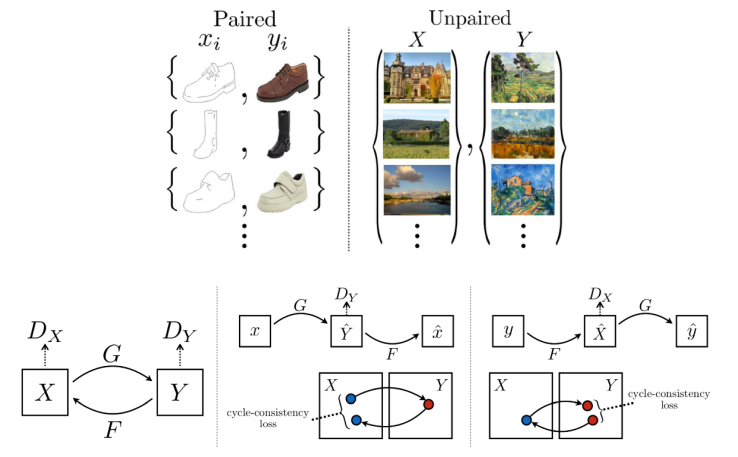
\includegraphics[height=0.7\textheight, width=\textwidth, keepaspectratio]{images/gan/cycle_gan_1.png}
\end{figure}
\framebreak
$$C_{horse \rightarrow zebra} = horse \rightarrow G_{horse \rightarrow zebra} \rightarrow \hat{zebra} \rightarrow [D_{zebra}, G_{zebra \rightarrow horse}] \rightarrow \hat{horse}$$
\begin{figure}
    \centering
    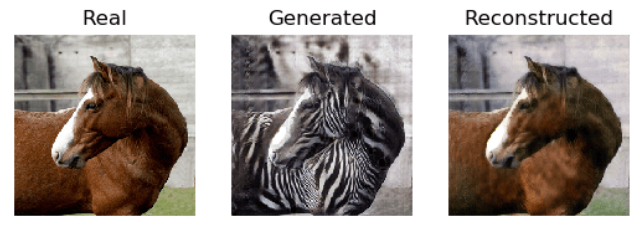
\includegraphics[height=0.7\textheight, width=\textwidth, keepaspectratio]{images/gan/cycle_gan_2.png}
\end{figure}

\framebreak
$$C_{zebra \rightarrow horse} = zebra \rightarrow G_{zebra \rightarrow horse} \rightarrow \hat{horse} \rightarrow [D_{horse}, G_{horse \rightarrow zebra}] \rightarrow \hat{zebra}$$
\begin{figure}
    \centering
    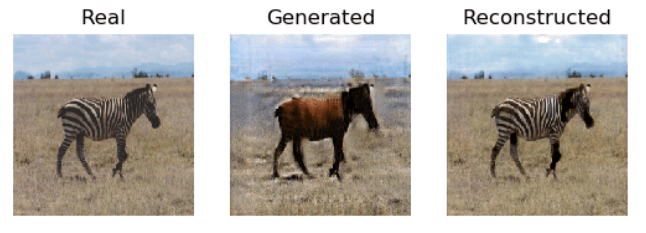
\includegraphics[height=0.7\textheight, width=\textwidth, keepaspectratio]{images/gan/cycle_gan_3.png}
\end{figure}

\framebreak
\begin{figure}
    \centering
    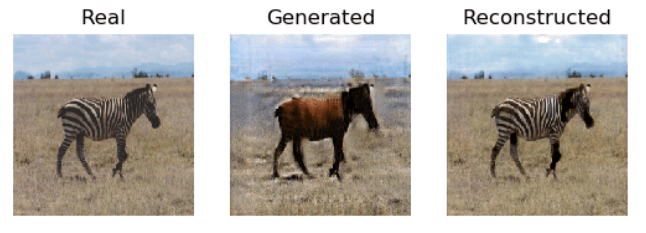
\includegraphics[height=0.7\textheight, width=\textwidth, keepaspectratio]{images/gan/cycle_gan_3.png}
\end{figure}

\framebreak
\begin{figure}
    \centering
    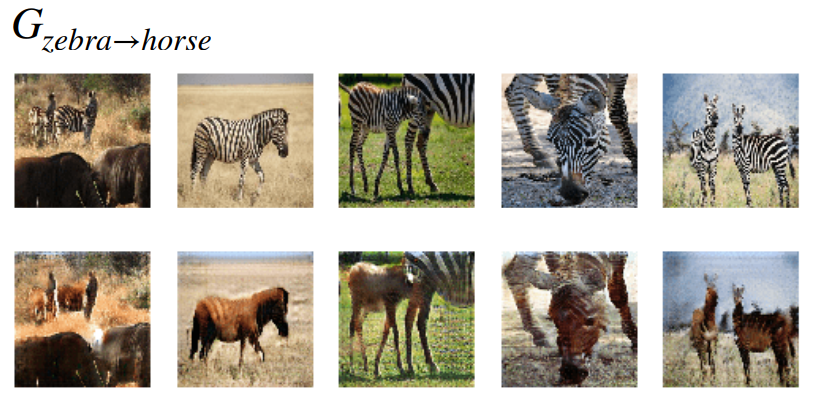
\includegraphics[height=0.9\textheight, width=\textwidth, keepaspectratio]{images/gan/cycle_gan_4.png}
\end{figure}

\framebreak
\begin{figure}
    \centering
    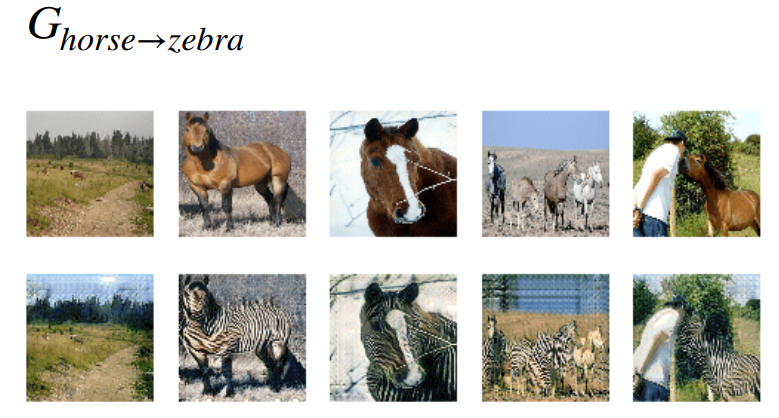
\includegraphics[height=0.9\textheight, width=\textwidth, keepaspectratio]{images/gan/cycle_gan_5.png}
\end{figure}

\framebreak
\begin{figure}
    \centering
    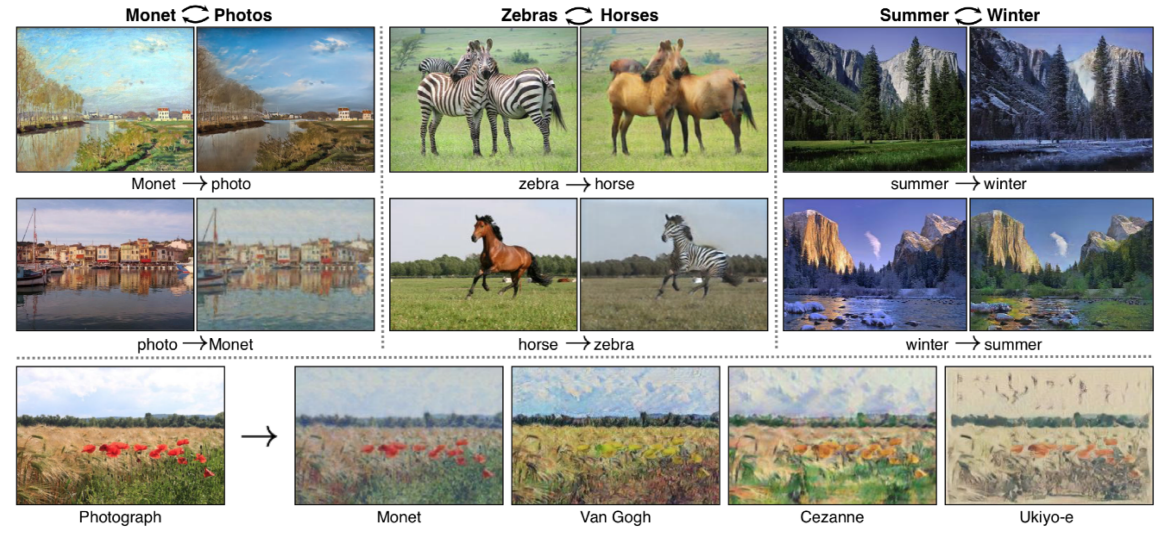
\includegraphics[height=0.9\textheight, width=\textwidth, keepaspectratio]{images/gan/cycle_gan_6.png}
    \caption{Image to Image translation with Cycle GANs}
\end{figure}
\end{frame}
\subsection{Style GANs}
\begin{frame}{}
    \LARGE GAN Variant: \\[1.5ex] \textbf{Style GANs}
\end{frame}

\begin{frame}[allowframebreaks]{Style GANs}
\begin{itemize}
    \item Goal: Better disentanglement of features in latent space (\textbf{W} space)
\end{itemize}
    \begin{figure}
    \centering
    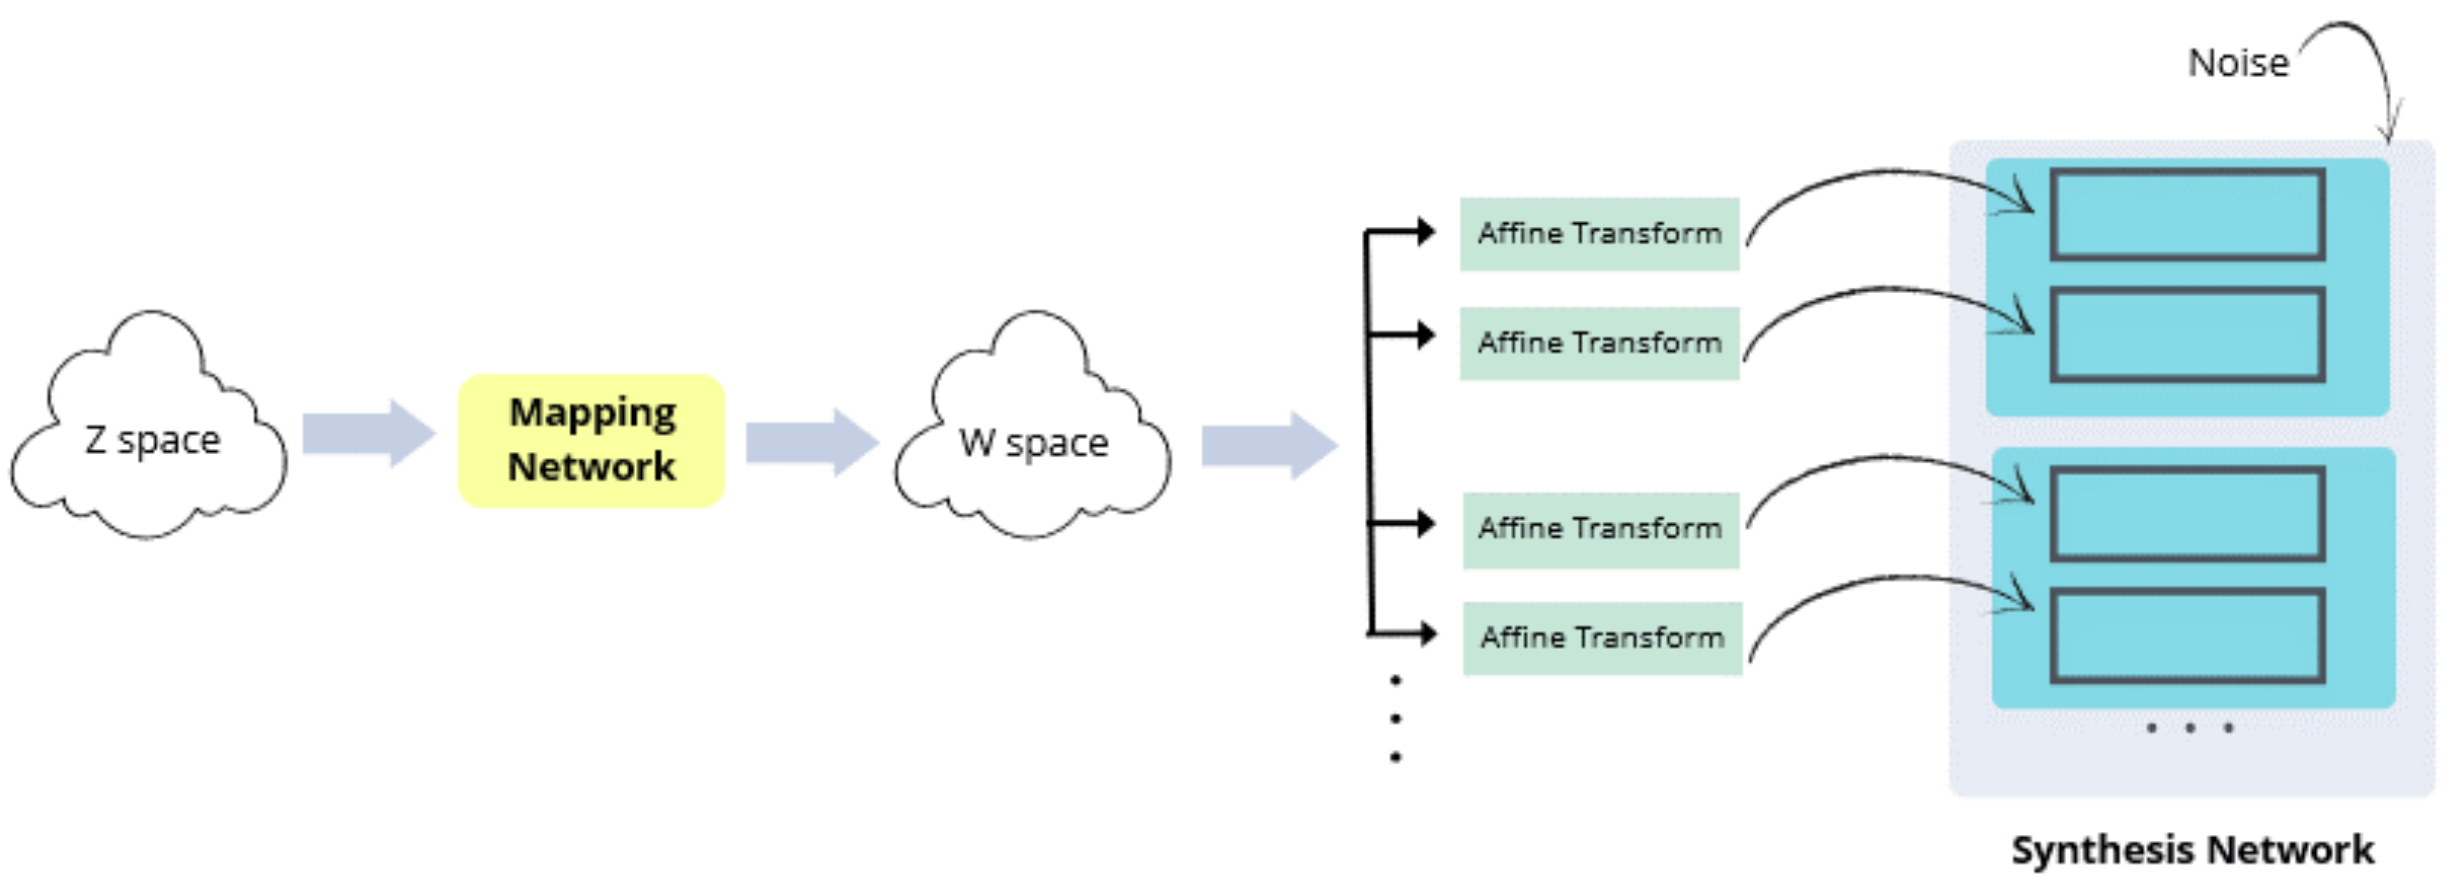
\includegraphics[height=0.9\textheight, width=\textwidth, keepaspectratio]{images/gan/stylegan_2.png}
\end{figure}

\footnotetext{https://www.cs.unc.edu/~ronisen/teaching/fall_2022/pdf_lectures/lecture6_gan2.pdf}
\end{frame}
\begin{frame}[allowframebreaks]{Style GANs}
\begin{figure}
    \centering
    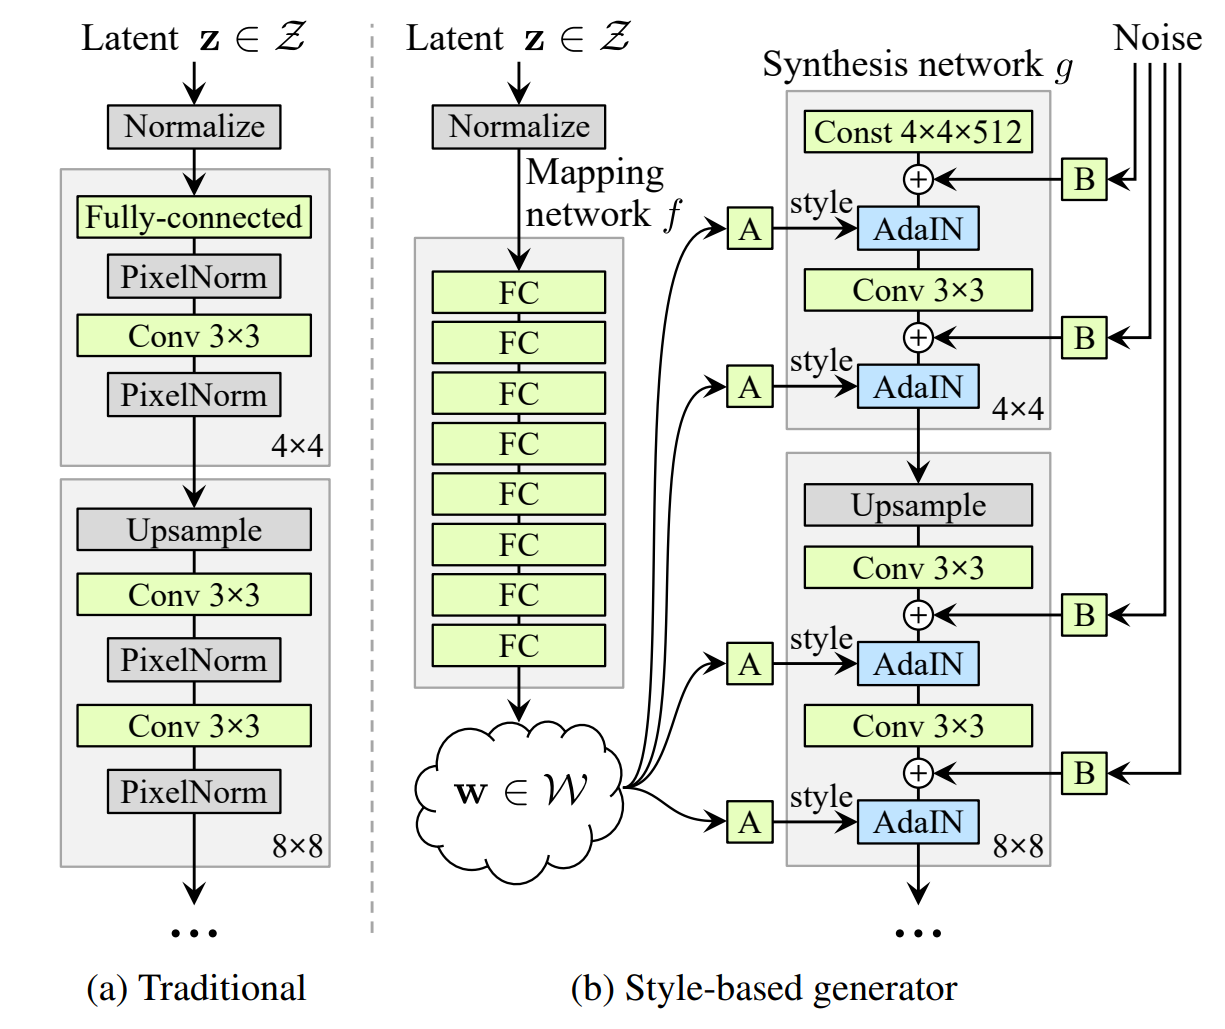
\includegraphics[height=0.9\textheight, width=\textwidth, keepaspectratio]{images/gan/stylegan_1.png}
\end{figure}
\footnotetext{https://arxiv.org/pdf/1812.04948}
\end{frame}
\begin{frame}[allowframebreaks]{Style GANs}

\begin{itemize}
    \item \textbf{A} = learned affine transformation block for AdaIN (predicts y)
    \item \textbf{Ada}ptive \textbf{I}stance \textbf{N}ormalization (very effective in controlling styles)
    $$\text{AdaIN}(x_i,y) = y_{s,i}\frac{x_i - u(x_i}{\sigma(x_i)} + y_{b,i}$$
    \item \textbf{B} = learned per-channel scaling factor for noise input.

\end{itemize}

\end{frame}

\begin{frame}[allowframebreaks]{Which Latent space to choose for embedding and editing?}
\begin{itemize}
    \item \textbf{Z} : 512 dimensional latent space (not good)
    \item \textbf{W} : 512 dimensional latent space (better but not perfect)
    \item \textbf{W+} : 18x512 dimensional latent space (after affine transformation \textbf{A} has been applied)
    \item \textbf{W} is better for editing.
    \item \textbf{W+} is better for reconstruction or embedding of real images.
\end{itemize}

\end{frame}

\begin{frame}[allowframebreaks]{Style GANs - Results}
\begin{figure}
    \centering
    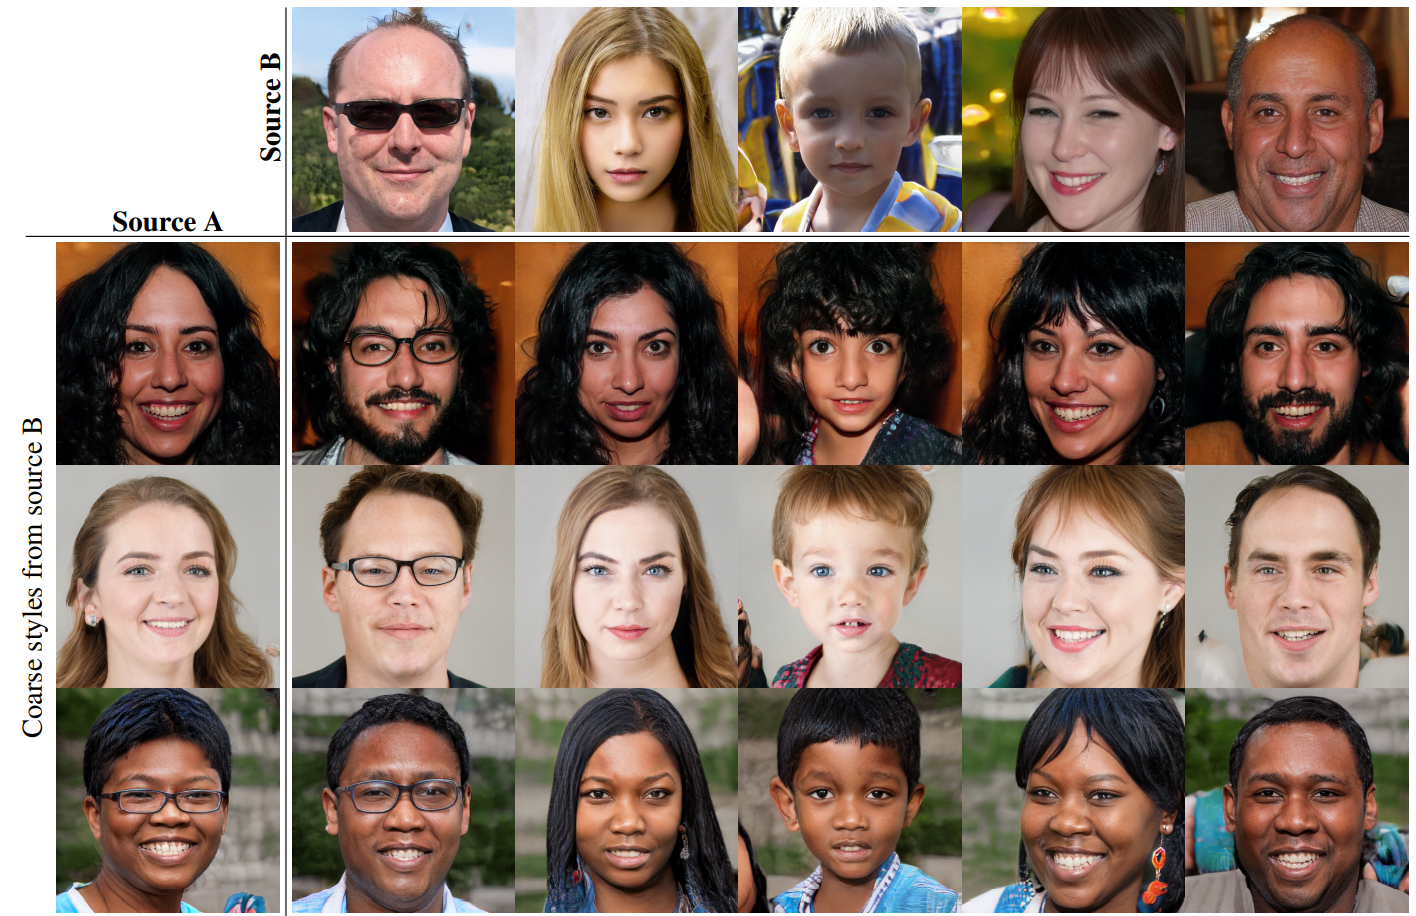
\includegraphics[height=0.9\textheight, width=\textwidth, keepaspectratio]{images/gan/stylegan_3.png}
\end{figure}
\footnotetext{https://arxiv.org/pdf/1812.04948}
\end{frame}